% ------------------------------------------------------------------------------
% Este fichero es parte de la plantilla LaTeX para la realización de Proyectos
% Final de Grado, protegido bajo los términos de la licencia GFDL.
% Para más información, la licencia completa viene incluida en el
% fichero fdl-1.3.tex

% Copyright (C) 2012 SPI-FM. Universidad de Cádiz
% ------------------------------------------------------------------------------

\documentclass[a4paper,11pt]{book}

% PAQUETES
\usepackage{./estilo/paquetes}
\usepackage{./estilo/colores}
\usepackage{./estilo/comandos}

% Ruta al directorio de imágenes
\graphicspath{{./img/}} 

% METADATOS
\title{Estudio Dietético Programado 2011//(EDP11)}
\author{Manuel González Pérez}
\date{Julio 2012} 
 
\begin{document}

\pagestyle{empty}

% PORTADAS
% ------------------------------------------------------------------------------
% Este fichero es parte de la plantilla LaTeX para la realización de Proyectos
% Final de Grado, protegido bajo los términos de la licencia GFDL.
% Para más información, la licencia completa viene incluida en el
% fichero fdl-1.3.tex

% Copyright (C) 2012 SPI-FM. Universidad de Cádiz
% ------------------------------------------------------------------------------


\begin{titlepage}

  \begin{center}

    
\includegraphics[width=0.3\textwidth]{logo-uca.png} \\
    
    \vspace{2.5cm}
    
    \LARGE{\textbf{ESCUELA SUPERIOR DE INGENIERÍA}} \\
    
    \vspace{1.0cm}
    
    \Large{\textbf{INGENIERÍA TÉCNICA EN INFORMÁTICA DE SISTEMAS}} \\
    
    \vspace{3.0cm}
    
    \Large{ESTUDIO DIETÉTICO PROGRAMADO 2011\\(EDP11)} \\
    
    \vspace{2.5cm}
    
    \Large{Manuel González Pérez} \\
  
    \vspace{0.5cm}

    \large{\today}
    
  \end{center}
\end{titlepage}

\cleardoublepage

% ------------------------------------------------------------------------------
% Este fichero es parte de la plantilla LaTeX para la realización de Proyectos
% Final de Grado, protegido bajo los términos de la licencia GFDL.
% Para más información, la licencia completa viene incluida en el
% fichero fdl-1.3.tex

% Copyright (C) 2012 SPI-FM. Universidad de Cádiz
% ------------------------------------------------------------------------------


\begin{center}

  
\includegraphics[width=0.3\textwidth]{logo-uca.png} \\

  \vspace{2.5cm}

  \Large{ESCUELA SUPERIOR DE INGENIERÍA} \\

  \vspace{1.0cm}

  \large{INGENIERÍA TÉCNICA EN INFORMÁTICA DE SISTEMAS} \\

  \vspace{2.0cm}

  \large{ESTUDIO DIETÉTICO PROGRAMADO 2011\\(EDP11)} \\

  \vspace{2.5cm}

\end{center}

\begin{itemize}
\item \large{Departamento: Lenguajes y Sistemas informáticos}
\item \large{Director y codirector del proyecto: Manuel Palomo Duarte e Iván Ruiz Rube}
\item \large{Autor del proyecto: Manuel González Pérez}
\end{itemize}

\vspace{0.2cm}

\begin{flushright}
  \large{Cádiz, \today} \\

  \vspace{2.5cm}

  \large{Fdo: Manuel González Pérez}
\end{flushright}

\cleardoublepage

% PRELIMINARES
% ------------------------------------------------------------------------------
% Este fichero es parte de la plantilla LaTeX para la realización de Proyectos
% Final de Grado, protegido bajo los términos de la licencia GFDL.
% Para más información, la licencia completa viene incluida en el
% fichero fdl-1.3.tex

% Copyright (C) 2012 SPI-FM. Universidad de Cádiz
% ------------------------------------------------------------------------------

\thispagestyle{empty}

\noindent \textbf{\begin{Large}\textit{Agradecimientos}\end{Large}} 
\newline
\newline
\noindent\textit{Agradecimientos a mis familiares por su apoyo, a mi novia por su paciencia y aguante, y a mi director de proyecto Manuel Palomo y codirector Ivan Ruiz, por su dedicación, aceptación e interés que han puesto.}

\newpage

% ------------------------------------------------------------------------------
% Este fichero es parte de la plantilla LaTeX para la realización de Proyectos
% Final de Grado, protegido bajo los términos de la licencia GFDL.
% Para más información, la licencia completa viene incluida en el
% fichero fdl-1.3.tex

% Copyright (C) 2012 SPI-FM. Universidad de Cádiz
% ------------------------------------------------------------------------------

\thispagestyle{empty}

\noindent \textbf{\begin{Large}Resumen\end{Large}} 
\newline
\newline
Programa de escritorio desarrollado a medida para una dietista, que observando el crecimiento de los pacientes a tratar y el tiempo dedicado para cada uno de ellos ha decidido informatizar su sistema de dietas y forma de gestión de los pacientes.\\\\
El programa constará de gestión de pacientes, gestión de recetas y alimentos, así como generación de dietas semanales acorde con el sistema de la interesada.\\
El programa se desarrollará bajo la tecnología \textit{Python} y para la parte gráfica \textit{Qt}, es decir, se desarrollará bajo \textit{PyQt}.\\\\
El código se realizará bajo la licencia \textit{GNU GPL 3.0} y para la documentación y memoria se usará \textit{GFDL 1.3}.

\newpage


\frontmatter

% INDICES
\tableofcontents
\listoffigures
\listoftables

\mainmatter

% PROLEGÓMENO
\part{Prolegómeno}
\null\vfill

\chapter{Introducción}
% ------------------------------------------------------------------------------
% Este fichero es parte de la plantilla LaTeX para la realización de Proyectos
% Final de Grado, protegido bajo los términos de la licencia GFDL.
% Para más información, la licencia completa viene incluida en el
% fichero fdl-1.3.tex

% Copyright (C) 2012 SPI-FM. Universidad de Cádiz
% ------------------------------------------------------------------------------

Este Proyecto Fin de Carrera tiene como objetivos: aplicar los conocimientos adquiridos durante la titulación Ingeniería Técnica en Informática de Sistemas, aprender y utilizar nuevas herramientas que enriquecen los conocimientos que no se han podido adquirir durante la titulación y aportar una contribución al mundo del Software Libre y al sector de la nutrición a la que esta orientado dicho proyecto.

\section{Motivación}
En el mundo de hoy, existen muchos problemas de salud, cada día siendo más comunes los problemas relacionados con la comida, como son la obesidad o el colesterol. Es por ello que se hace más necesario personas que nos orienten en cuanto a alimentación nos referimos, tales como los nutricionistas.\\
Por este motivo es por el que se desarrolla dicho proyecto, para hacer más fácil la tarea de los nutricionistas, informatizando sus sistemas y ahorrándoles tiempo y esfuerzo.

\section{Objetivos y alcance del proyecto} 
Este proyecto consiste en la creación de un software que permita gestionar los hábitos alimenticios de los pacientes, así como la posibilidad de gestionar una pequeña o mediana empresa de nutricionistas, como son las franquicias de nutrición más conocidas, albergando el numeroso personal de nutricionistas que tienen al frente.\\

Como objetivos se plantean:\\
\begin{itemize}
\item Gestión de Dietistas
\item Gestión de Pacientes
\item Gestión de Recetas
\item Gestión de Ingredientes
\item Gestión de Semanarios
\end{itemize}


\section{Organización del documento}
Este documento se compone de:
\begin{itemize}
\item \textbf{Introducción}: pequeña descripción del proyecto, incluyendo objetivos, alcance y estructura.
\item \textbf{Planificación}: planificación temporal para el desarrollo del proyecto, reflejándola mediante un diagrama de "Gantt".
\item \textbf{Análisis}: análisis del sistema. Definiéndose los requisitos funcionales, diagramas de casos de uso, diagramas de secuencia y contrato de operaciones.
\item \textbf{Diseño}: diseño del sistema. Obteniéndose la base de datos, diagramas de secuencia y de clases aplicadas al diseño.
\item \textbf{Implementación}: se detallarán algunos aspectos relevantes para la implementación así como la superación de posibles problemas que se pudieran encontrar durante la implementación.
\item \textbf{Pruebas y Validaciones}: pruebas realizadas para la corroboración del funcionamiento del software.
\item \textbf{Manual de Usuario}: manual para el uso de la aplicación.
\item \textbf{Manual de instalación y explotación}: manual para la instalación de la aplicación. 
\item \textbf{Conclusiones}: valoración personal de la realización del proyecto y futuras mejoras.
\item \textbf{Bibliografía}: referencias, enlaces, libros y ayudas consultadas durante el desarrollo del proyecto.
\item \textbf{Información sobre Licencia}: licencia en la que se basa el proyecto, en concreto, GPL 3.0 y FDL 1.3.
\end{itemize}






\chapter{Planificación}
% ------------------------------------------------------------------------------
% Este fichero es parte de la plantilla LaTeX para la realización de Proyectos
% Final de Grado, protegido bajo los términos de la licencia GFDL.
% Para más información, la licencia completa viene incluida en el
% fichero fdl-1.3.tex

% Copyright (C) 2012 SPI-FM. Universidad de Cádiz
% ------------------------------------------------------------------------------


\section{Metodología de desarrollo}
El modelo de ciclo de vida empleado en el desarrollo del proyecto es el modelo incremental. Este modelo combina elementos del modelo lineal secuencial aplicado repetidamente conjunto a la filosofía de contrucción de prototipos.\\
Cuando se utiliza el modelo incremental en el primer incremento se afrontan requisitos básicos pero muchas funciones suplementarias quedan sin extraer. Como resultado del primer incremento se produce el producto central, el cual posteriormente de la utilización y/o evaluación se modifica a fin de cumplir todos los requisitos y necesidades del cliente.\\

\section{Planificación del proyecto}
La planificación temporal estimada que se ha llevado a cabo durante el desarrollo del proyecto es el siguiente:\\
\begin{itemize}
\item \textbf{Fase de Inicio (18/05/11 - 15/06/11)}: Durante esta etapa se plantea la idea y se consulta con los tutores si es adecuada y la disponibilidad.\\
\item \textbf{Fase de Desarrollo (16/06/11 - 09/08/12)}: Durante esta etapa se desarrolla el proyecto.
\begin{itemize}
\item \textbf{Especificación de requisitos (16/06/11 - 29/07/11)}: La toma de requisitos fue una labor compleja, debido a los constantes cambios y añadidos de funcionalidades. Finalmente se determinaron con éxito todas las funcionalidades y exigencias para el proyecto.
\item \textbf{Análisis (01/08/11 - 12/10/11)}: Teniendo los requisitos bien definidos el análisis ha sido más claro aunque también duradero.
\item \textbf{Diseño (13/10/11 - 30/01/12)}: Así como la implementación, ambas han sido las etapas que más tiempo han consumido. Esta etapa se ha hecho con especial cuidado de realizar un diseño correcto para no interrumpir la implementación por posibles errores.
\item \textbf{Implementación (30/01/12 - 12/07/12)}: Dicha etapa ha sido la más larga durante el desarrollo, en la que se han implementado todos los requisitos satisfaciendo las necesidades previstas.
\item \textbf{Pruebas (13/07/12 - 09/08/12)}: Se han probado todas las funcionalidades comprobando su correcto funcionamiento y ejecución, asegurándose que no hay ningún tipo de error.
\end{itemize}
\item \textbf{Fase de Documentación (10/08/12 - 03/12/12)}: En esta etapa se redactó este documento y todos los necesarios para el complemento del proyecto.
\end{itemize}

Esta planificación se observa mejor en el siguiente diagrama de Gantt.\\
Para mayor legibilidad del diagrama de Gantt, se omite en éste las entregas del producto esencial (o primer incremento), así como sus posteriores incrementos\\
Para realizar el diagrama de ``Gantt'', se ha utilizado la herramienta \textit{Gantt Project}.\\

\begin{figure}[H]
  \label{finicio}
  \begin{center}
    % Comentar si no está el paquete tkiz instalado, y descomentar la
    % linea siguiente. Comentar además la inclusión del paquete en
    % estilos/estiloBase.sty
    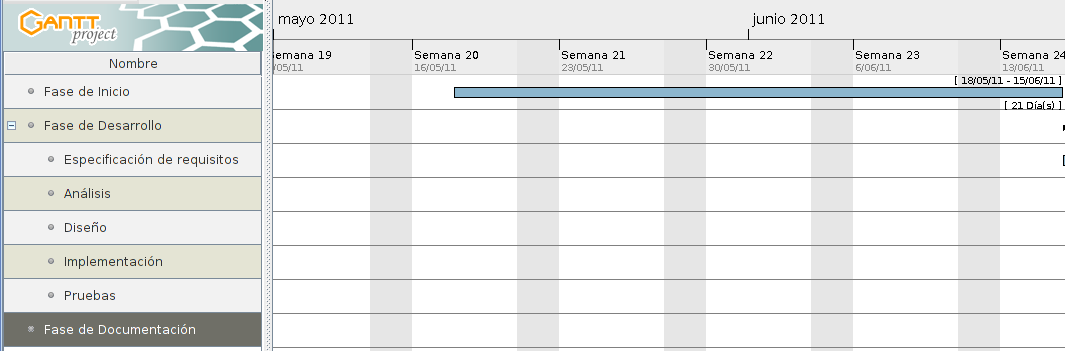
\includegraphics[scale=0.4]{../img/fase-inicio.png} 
  \end{center}
  \caption{Diagrama de Gantt: Fase de Inicio}
\end{figure}

\begin{figure}[H]
  \label{fdes}
  \begin{center}
    % Comentar si no está el paquete tkiz instalado, y descomentar la
    % linea siguiente. Comentar además la inclusión del paquete en
    % estilos/estiloBase.sty
    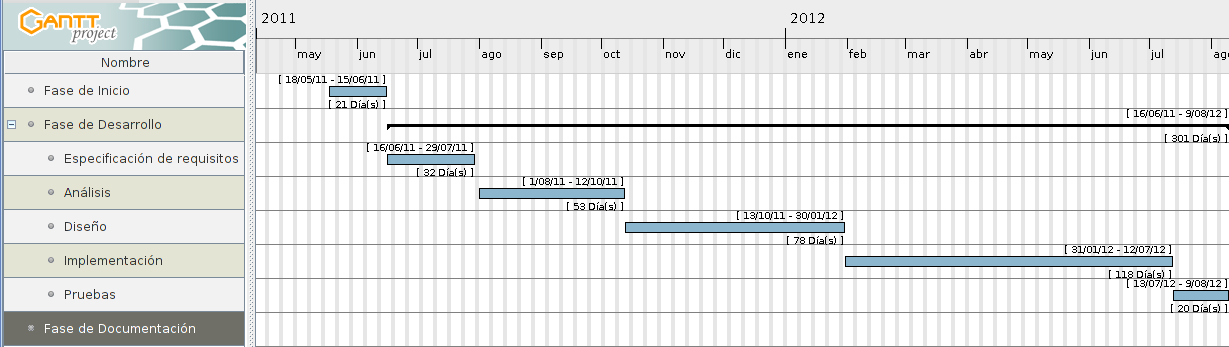
\includegraphics[scale=0.4]{../img/fase-desarrollo.png} 
  \end{center}
  \caption{Diagrama de Gantt: Fase de Desarrollo}
\end{figure}

\begin{figure}[H]
  \label{fdoc}
  \begin{center}
    % Comentar si no está el paquete tkiz instalado, y descomentar la
    % linea siguiente. Comentar además la inclusión del paquete en
    % estilos/estiloBase.sty
    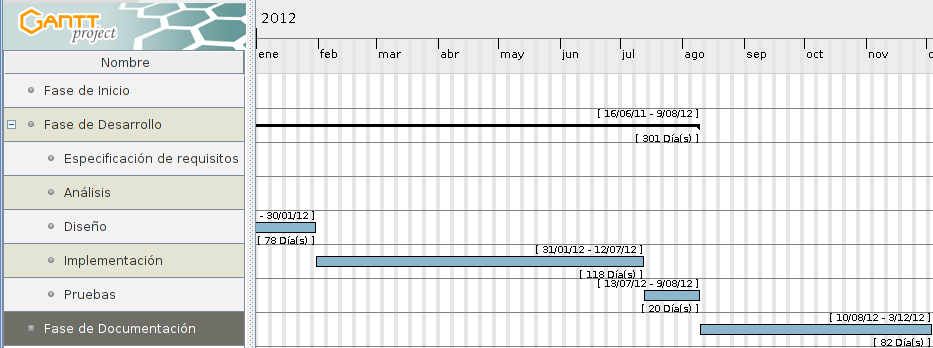
\includegraphics[scale=0.5]{../img/fase-documentacion.png} 
  \end{center}
  \caption{Diagrama de Gantt: Fase de Documentación}
\end{figure}

% DESARROLLO
\part{Desarrollo}
\null\vfill

\chapter{Análisis de Requisitos}
% ------------------------------------------------------------------------------
% Este fichero es parte de la plantilla LaTeX para la realización de Proyectos
% Final de Grado, protegido bajo los términos de la licencia GFDL.
% Para más información, la licencia completa viene incluida en el
% fichero fdl-1.3.tex

% Copyright (C) 2012 SPI-FM. Universidad de Cádiz
% ------------------------------------------------------------------------------

\section{Catálogo de actores}
Los usuarios que interactúan con el sistema se diferencian en actores, en este caso, dietista, paciente y administrador.
\begin{itemize}
\item \textbf{Dietista:} Este actor será el responsable directo de la interactuación con la aplicación, siendo responsable de todos los requisitos funcionales.
\item \textbf{Paciente:} Este actor intervendrá en algunos de los requisitos y será el mayor beneficiario de la aplicación.
\item \textbf{Administrador:} Este actor sólo intervendrá en el caso de uso \textit{Eliminar Perfil Dietista}, siendo necesario para poder llevarse a cabo la acción.
\end{itemize}

\section{Requisitos funcionales}
A continuación se exponen los requisitos funcionales de la aplicación:
\begin{itemize}
\item \textbf{Requisitos funcionales de la gestión de dietistas:}
\begin{itemize}
\item Se podrá añadir un nuevo dietista a la aplicación registrando sus propios datos.
\item Se podrá abrir un perfil de dietista existente, previamente registrado, y suministrando la clave correspondiente.
\item Se podrá cerrar un perfil de dietista abierto previamente.
\item Se podrá eliminar un perfil de dietista existente.
\end{itemize}
\item \textbf{Requisitos funcionales de la gestión de pacientes:}
\begin{itemize}
\item Se podrá añadir un nuevo paciente a la aplicación, registrando el dietista los datos de dicho paciente.
\item Se podrá abrir un perfil de paciente existente y perteneciente al dietista actualmente en uso de la aplicación.
\item Se podrán editar los datos de un perfil de paciente una vez abierto mediante el botón guardar.
\item Se podrá cerrar un perfil de paciente abierto previamente.
\item Se podrá eliminar un perfil de paciente existente y perteneciente al dietista actualmente en uso de la aplicación.
\item Se podrá añadir y modificar información médica referente al paciente, tales como analíticas, tratamiento farmacológico o enfermedades/patologías.
\item Se podrá añadir información general referente al paciente.
\item Se podrán añadir diarios dietéticos rellenados por el paciente.
\item Se podrán eliminar diarios dietéticos de un paciente.
\item Se podrán añadir recordatorios 24h. rellenados por el paciente.
\item Se podrán eliminar recordatorios 24h. de un paciente.
\item Se podrá añadir la frecuencia de ingesta de alimentos de un paciente.
\item Se podrán añadir recetas al semanario del paciente en uso.
\item Se podrán ver los semanarios existentes del paciente en uso.
\end{itemize}
\item \textbf{Requisitos funcionales de la gestión de recetas:}
\begin{itemize}
\item Se podrán añadir nuevas recetas de un dietista en uso.
\item Se podrán editar recetas existentes de un dietista en uso.
\item Se podrán eliminar recetas existentes de un dietista en uso.
\end{itemize}
\end{itemize}

\section{Análisis}
\subsection{Modelos de casos de uso}
A continuación se muestran las especificaciones de casos de uso, con sus respectivos diagramas.
\subsubsection{Casos de uso respecto a la gestión de dietistas}
\begin{figure}[H]
  \label{cu_dietista}
  \begin{center}
    % Comentar si no está el paquete tkiz instalado, y descomentar la
    % linea siguiente. Comentar además la inclusión del paquete en
    % estilos/estiloBase.sty
    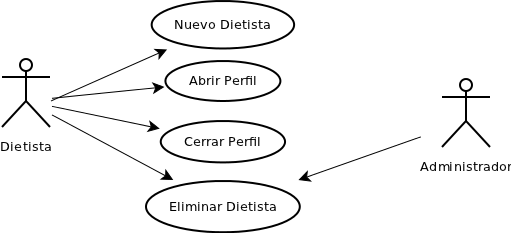
\includegraphics[scale=0.7]{../img/CU_Dietista.png}
  \end{center}
  \caption{Diagrama de caso de uso: Gestión de dietistas}
\end{figure}

\textbf{Caso de Uso: Nuevo Dietista}
\begin{itemize}
\item \textbf{Descripción:} Resgistro de dietista en el sistema.
\item \textbf{Precondición:} El dietista no existe en el sistema.
\item \textbf{Postcondición:} El dietista se registra en el sistema.
\item \textbf{Actores:} Dietista(principal)
\item \textbf{Resumen:} El dietista desea darse de alta en el sistema.
\item \textbf{Escenario Principal:}
\begin{enumerate}
\item El dietista solicita al sistema darse de alta.
\item El dietista rellena los datos solicitados.
\item El sistema comprueba los datos introducidos.
\item Se almacenan los datos en el sistema.
\end{enumerate}
\item \textbf{Escenario Alternativo:}
\begin{enumerate}
\item[0] En cualquier momento el dietista puede cancelar el proceso.
\item[3] Existen campos vacíos o erróneos. Mensajes de advertencia sobre los campos afectados.
\item[3a] Existe un dietista con el mismo DNI. Mensaje de advertencia del sistema.
\end{enumerate}
\end{itemize}
\begin{figure}[H]
  \label{ds_nuevodietista}
  \begin{center}
    % Comentar si no está el paquete tkiz instalado, y descomentar la
    % linea siguiente. Comentar además la inclusión del paquete en
    % estilos/estiloBase.sty
    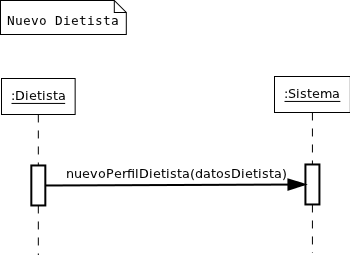
\includegraphics[scale=0.7]{../img/DS_NuevoDietista.png}
  \end{center}
  \caption{Diagrama de secuencia: Nuevo Dietista}
\end{figure}
\textbf{Contrato de la operación:} nuevoPerfilDietista(datosDietista)
\begin{itemize}
\item \textbf{Responsabilidades:} Registrar un nuevo dietista en el sistema.
\item \textbf{Referencias cruzadas:} Caso de uso ``Nuevo Dietista''.
\item \textbf{Precondición:}
\begin{itemize}
\item El dietista no se encuentra registrado en el sistema.
\item datosDietista es válido.
\end{itemize}
\item \textbf{Postcondición:}
\begin{itemize}
\item El dietista se guarda en el sistema.
\end{itemize}
\end{itemize}

\textbf{Caso de Uso: Abrir Perfil}
\begin{itemize}
\item \textbf{Descripción:} Abrir perfil de dietista solicitado.
\item \textbf{Precondición:} El dietista existe en el sistema.
\item \textbf{Postcondición:} El dietista abre perfil en el sistema.
\item \textbf{Actores:} Dietista(principal)
\item \textbf{Resumen:} El dietista desea abrir su perfil en el sistema.
\item \textbf{Escenario Principal:}
\begin{enumerate}
\item El dietista solicita al sistema abrir su perfil.
\item El dietista rellena la clave que se le solicita.
\item El sistema comprueba la clave introducida.
\item Se abre el perfil del dietista en el sistema.
\end{enumerate}
\item \textbf{Escenario Alternativo:}
\begin{enumerate}
\item[0] En cualquier momento el dietista puede cancelar el proceso.
\item[3] La clave es errónea. Mensaje de advertencia del sistema.
\end{enumerate}
\end{itemize}
\begin{figure}[H]
  \label{ds_abrirdietista}
  \begin{center}
    % Comentar si no está el paquete tkiz instalado, y descomentar la
    % linea siguiente. Comentar además la inclusión del paquete en
    % estilos/estiloBase.sty
    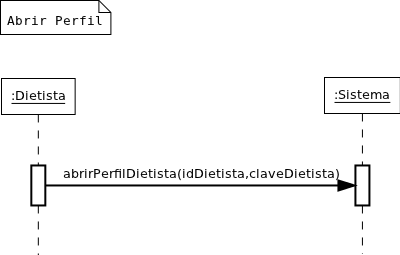
\includegraphics[scale=0.7]{../img/DS_AbrirDietista.png}
  \end{center}
  \caption{Diagrama de secuencia: Abrir Perfil Dietista}
\end{figure}
\textbf{Contrato de la operación:} abrirPerfilDietista(idDietista,claveDietista)
\begin{itemize}
\item \textbf{Responsabilidades:} Abrir perfil de dietista en el sistema.
\item \textbf{Referencias cruzadas:} Caso de uso ``Abrir Perfil''.
\item \textbf{Precondición:}
\begin{itemize}
\item Existe un dietista con id = idDietista.
\item claveDietista es válida.
\end{itemize}
\item \textbf{Postcondición:}
\begin{itemize}
\item El sistema carga los datos del dietista en el sistema.
\end{itemize}
\end{itemize}

\textbf{Caso de Uso: Cerrar Perfil}
\begin{itemize}
\item \textbf{Descripción:} Cerrar perfil de dietista en uso del sistema.
\item \textbf{Precondición:} El dietista tiene abierto su perfil en el sistema.
\item \textbf{Postcondición:} El dietista cierra su perfil en el sistema.
\item \textbf{Actores:} Dietista(principal)
\item \textbf{Resumen:} El dietista desea cerrar su perfil en el sistema.
\item \textbf{Escenario Principal:}
\begin{enumerate}
\item El dietista solicita al sistema cerrar su perfil.
\item El sistema cierra el perfil del dietista.
\item Se cierra el perfil del dietista en el sistema.
\end{enumerate}
\item \textbf{Escenario Alternativo:}
\begin{enumerate}
\item[0] En cualquier momento el dietista puede cancelar el proceso.
\end{enumerate}
\end{itemize}
\begin{figure}[H]
  \label{ds_cerrardietista}
  \begin{center}
    % Comentar si no está el paquete tkiz instalado, y descomentar la
    % linea siguiente. Comentar además la inclusión del paquete en
    % estilos/estiloBase.sty
    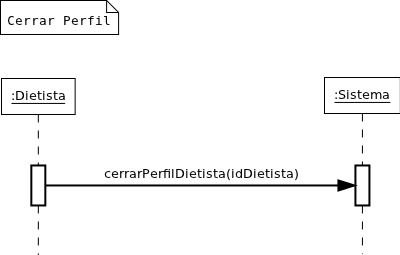
\includegraphics[scale=0.7]{../img/DS_CerrarDietista.png}
  \end{center}
  \caption{Diagrama de secuencia: Cerrar Perfil Dietista}
\end{figure}
\textbf{Contrato de la operación:} cerrarPerfilDietista(idDietista)
\begin{itemize}
\item \textbf{Responsabilidades:} Cerrar perfil de dietista en el sistema.
\item \textbf{Referencias cruzadas:} Caso de uso ``Cerrar Perfil''.
\item \textbf{Precondición:}
\begin{itemize}
\item Existe un Dietista D con D.id = idDiestista en uso.
\end{itemize}
\item \textbf{Postcondición:}
\begin{itemize}
\item El sistema cierra el perfil del dietista en el sistema.
\end{itemize}
\end{itemize}

\textbf{Caso de Uso: Eliminar Dietista}
\begin{itemize}
\item \textbf{Descripción:} Eliminar perfil de dietista del sistema.
\item \textbf{Precondición:} El dietista existe y no tiene abierto su perfil en el sistema.
\item \textbf{Postcondición:} El dietista elimina su perfil del sistema.
\item \textbf{Actores:} Dietista(principal) y Administrador(secundario)
\item \textbf{Resumen:} El dietista desea eliminar su perfil del sistema.
\item \textbf{Escenario Principal:}
\begin{enumerate}
\item El dietista solicita al sistema eliminar su perfil.
\item El dietista solicita al administrador la clave de confirmación y la introduce.
\item El sistema comprueba la clave de confimación.
\item Se elimina el perfil del dietista del sistema.
\end{enumerate}
\item \textbf{Escenario Alternativo:}
\begin{enumerate}
\item[0] En cualquier momento el dietista puede cancelar el proceso.
\item[3] La clave de confirmación es errónea. Mensaje de advertencia del sistema.
\end{enumerate}
\end{itemize}
\begin{figure}[H]
  \label{ds_eliminardietista}
  \begin{center}
    % Comentar si no está el paquete tkiz instalado, y descomentar la
    % linea siguiente. Comentar además la inclusión del paquete en
    % estilos/estiloBase.sty
    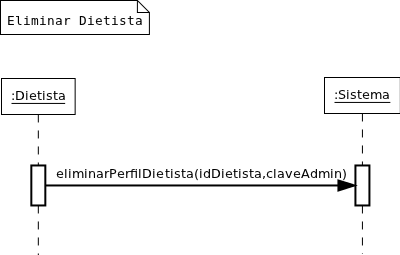
\includegraphics[scale=0.7]{../img/DS_EliminarDietista.png}
  \end{center}
  \caption{Diagrama de secuencia: Eliminar Dietista}
\end{figure}
\textbf{Contrato de la operación:} eliminarPerfilDietista(idDiestista, claveAdmin)
\begin{itemize}
\item \textbf{Responsabilidades:} Eliminar perfil de dietista del sistema.
\item \textbf{Referencias cruzadas:} Caso de uso ``Eliminar Dietista''.
\item \textbf{Precondición:}
\begin{itemize}
\item Existe un dietista con id = idDietista.
\item claveAdmin es válido.
\end{itemize}
\item \textbf{Postcondición:}
\begin{itemize}
\item Se eliminan los datos del dietista con idDietista.
\end{itemize}
\end{itemize}


\newpage
\subsubsection{Casos de uso respecto a la gestión de pacientes}
\begin{figure}[H]
  \label{cu_paciente}
  \begin{center}
    % Comentar si no está el paquete tkiz instalado, y descomentar la
    % linea siguiente. Comentar además la inclusión del paquete en
    % estilos/estiloBase.sty
    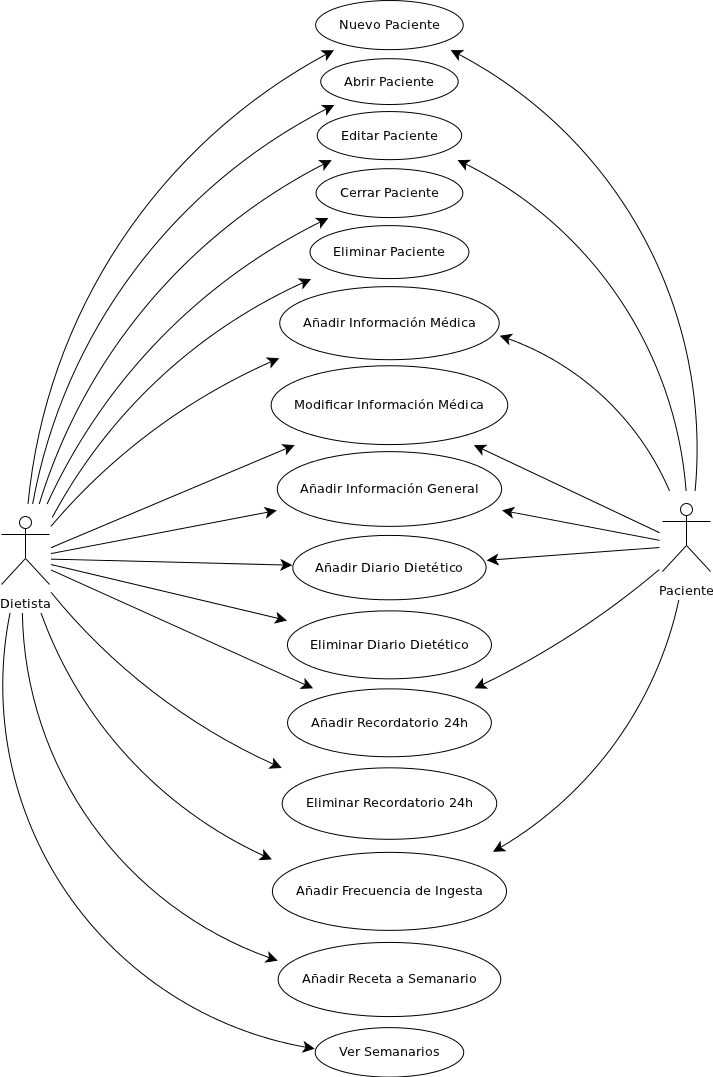
\includegraphics[scale=0.6]{../img/CU_Paciente.png}
  \end{center}
  \caption{Diagrama de caso de uso: Gestión de pacientes}
\end{figure}

\textbf{Caso de Uso: Nuevo Paciente}
\begin{itemize}
\item \textbf{Descripción:} Resgistro de un nuevo paciente en el sistema.
\item \textbf{Precondición:} El dietista existe y el paciente no existe en el sistema.
\item \textbf{Postcondición:} El paciente se registra en el sistema.
\item \textbf{Actores:} Dietista(principal)
\item \textbf{Resumen:} El dietista desea dar de alta un nuevo paciente en el sistema.
\item \textbf{Escenario Principal:}
\begin{enumerate}
\item El dietista solicita al sistema dar de alta un nuevo paciente.
\item El dietista rellena los datos solicitados del paciente.
\item El sistema comprueba los datos introducidos.
\item Se almacenan los datos en el sistema.
\end{enumerate}
\item \textbf{Escenario Alternativo:}
\begin{enumerate}
\item[0] En cualquier momento el dietista puede cancelar el proceso.
\item[3] Existen campos vacíos o erróneos. Mensajes de advertencia sobre los campos afectados.
\item[3a] Existe un paciente con el mismo DNI. Mensaje de advertencia del sistema.
\end{enumerate}
\end{itemize}
\begin{figure}[H]
  \label{ds_nuevopaciente}
  \begin{center}
    % Comentar si no está el paquete tkiz instalado, y descomentar la
    % linea siguiente. Comentar además la inclusión del paquete en
    % estilos/estiloBase.sty
    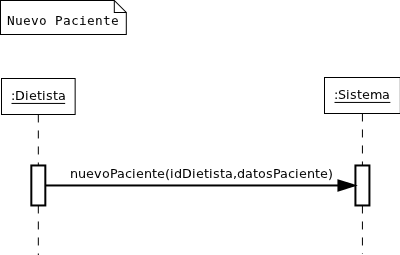
\includegraphics[scale=0.7]{../img/DS_NuevoPaciente.png}
  \end{center}
  \caption{Diagrama de secuencia: Nuevo Paciente}
\end{figure}
\textbf{Contrato de la operación:} nuevoPaciente(idDietista,datosPaciente)
\begin{itemize}
\item \textbf{Responsabilidades:} Registrar un nuevo paciente de un dietista en el sistema.
\item \textbf{Referencias cruzadas:} Caso de uso ``Nuevo Paciente''.
\item \textbf{Precondición:}
\begin{itemize}
\item Existe un dietista con id = idDietista en uso del sistema.
\item El paciente no existe en el sistema.
\item datosPaciente es válido.
\end{itemize}
\item \textbf{Postcondición:}
\begin{itemize}
\item El paciente se guarda en el sistema.
\end{itemize}
\end{itemize}

\textbf{Caso de Uso: Abrir Perfil Paciente}
\begin{itemize}
\item \textbf{Descripción:} Abrir perfil de un paciente en el sistema.
\item \textbf{Precondición:} El dietista y el paciente existen en el sistema.
\item \textbf{Postcondición:} El perfil del paciente se abre en el sistema.
\item \textbf{Actores:} Dietista(principal)
\item \textbf{Resumen:} El dietista desea abrir un perfil de un paciente en el sistema.
\item \textbf{Escenario Principal:}
\begin{enumerate}
\item El dietista solicita al sistema abrir un perfil de un paciente.
\item El sistema muestra el listado de pacientes existente, pertenecientes al dietista que lo solicita.
\item El dietista selecciona el perfil del paciente a abrir.
\item Se abre el perfil del paciente en el sistema.
\end{enumerate}
\item \textbf{Escenario Alternativo:}
\begin{enumerate}
\item[0] En cualquier momento el dietista puede cancelar el proceso.
\end{enumerate}
\end{itemize}
\begin{figure}[H]
  \label{ds_abrirpaciente}
  \begin{center}
    % Comentar si no está el paquete tkiz instalado, y descomentar la
    % linea siguiente. Comentar además la inclusión del paquete en
    % estilos/estiloBase.sty
    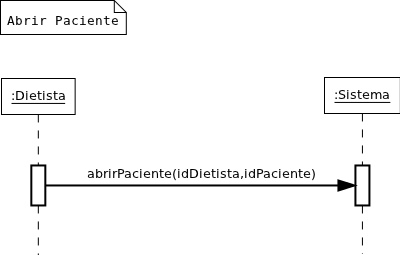
\includegraphics[scale=0.7]{../img/DS_AbrirPaciente.png}
  \end{center}
  \caption{Diagrama de secuencia: Abrir Perfil Paciente}
\end{figure}
\textbf{Contrato de la operación:} abrirPaciente(idDietista,idPaciente)
\begin{itemize}
\item \textbf{Responsabilidades:} Abrir un perfil de un paciente del dietista en el sistema.
\item \textbf{Referencias cruzadas:} Caso de uso ``Abrir Perfil Paciente''.
\item \textbf{Precondición:}
\begin{itemize}
\item El dietista con id = idDietista tiene su perfil abierto.
\item Existe un paciente con id = idPaciente.
\end{itemize}
\item \textbf{Postcondición:}
\begin{itemize}
\item El paciente con idPaciente se abre en el sistema.
\end{itemize}
\end{itemize}


\textbf{Caso de Uso: Editar Perfil Paciente}
\begin{itemize}
\item \textbf{Descripción:} Editar perfil de un paciente del sistema.
\item \textbf{Precondición:} El dietista y el paciente existen en el sistema.
\item \textbf{Postcondición:} El perfil del paciente se edita en el sistema.
\item \textbf{Actores:} Dietista(principal)
\item \textbf{Resumen:} El dietista desea editar el perfil de un paciente del sistema.
\item \textbf{Escenario Principal:}
\begin{enumerate}
\item El dietista solicita al sistema editar el perfil de un paciente.
\item El dietista presiona el botón guardar.
\item El sistema guarda los nuevos datos.
\end{enumerate}
\item \textbf{Escenario Alternativo:}
\begin{enumerate}
\item[2] El dietista no presiona el botón, los datos nuevos se perderán.
\end{enumerate}
\end{itemize}
\begin{figure}[H]
  \label{ds_editarpaciente}
  \begin{center}
    % Comentar si no está el paquete tkiz instalado, y descomentar la
    % linea siguiente. Comentar además la inclusión del paquete en
    % estilos/estiloBase.sty
    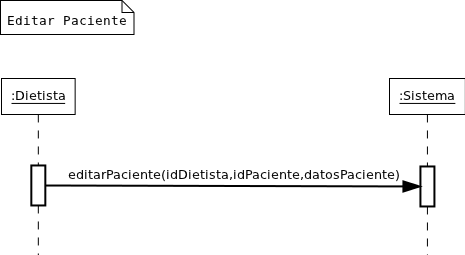
\includegraphics[scale=0.7]{../img/DS_EditarPaciente.png}
  \end{center}
  \caption{Diagrama de secuencia: Editar Datos Paciente}
\end{figure}
\textbf{Contrato de la operación:} editarPaciente(idDietista,idPaciente,datosPaciente)
\begin{itemize}
\item \textbf{Responsabilidades:} Editar el perfil de un paciente del dietista en el sistema.
\item \textbf{Referencias cruzadas:} Caso de uso ``Editar Perfil Paciente''.
\item \textbf{Precondición:}
\begin{itemize}
\item El dietista con id = idDietista tiene su perfil abierto.
\item El paciente con id = idPaciente tiene su perfil abierto.
\item datosPaciente es válido.
\end{itemize}
\item \textbf{Postcondición:}
\begin{itemize}
\item El paciente se edita en el sistema.
\end{itemize}
\end{itemize}

\textbf{Caso de Uso: Cerrar Perfil Paciente}
\begin{itemize}
\item \textbf{Descripción:} Cerrar perfil de paciente del sistema.
\item \textbf{Precondición:} El dietista y el paciente existen en el sistema.
\item \textbf{Postcondición:} El perfil del paciente se abre en el sistema.
\item \textbf{Actores:} Dietista(principal)
\item \textbf{Resumen:} El dietista desea cerrar el perfil de un paciente del sistema.
\item \textbf{Escenario Principal:}
\begin{enumerate}
\item El dietista solicita al sistema cerrar un perfil de un paciente.
\item El sistema solicita confirmación.
\item El dietista da la confirmación al cierre del perfil.
\item Se cierra el perfil del paciente en el sistema.
\end{enumerate}
\item \textbf{Escenario Alternativo:}
\begin{enumerate}
\item[0] En cualquier momento el dietista puede cancelar el proceso.
\item[3] El dietista no da la confirmación.
\item[3a] Se cancela el proceso.
\end{enumerate}
\end{itemize}
\begin{figure}[H]
  \label{ds_cerrarpaciente}
  \begin{center}
    % Comentar si no está el paquete tkiz instalado, y descomentar la
    % linea siguiente. Comentar además la inclusión del paquete en
    % estilos/estiloBase.sty
    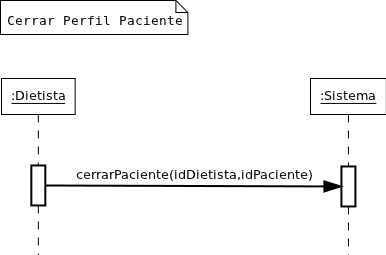
\includegraphics[scale=0.7]{../img/DS_CerrarPaciente.png}
  \end{center}
  \caption{Diagrama de secuencia: Cerrar Perfil Paciente}
\end{figure}
\textbf{Contrato de la operación:} cerrarPaciente(idDietista,idPaciente)
\begin{itemize}
\item \textbf{Responsabilidades:} Cerrar el perfil de un paciente del dietista en el sistema.
\item \textbf{Referencias cruzadas:} Caso de uso ``Cerrar Perfil Paciente''.
\item \textbf{Precondición:}
\begin{itemize}
\item El dietista con id = idDietista tiene su perfil abierto.
\item El paciente con id = idPaciente tiene su perfil abierto.
\end{itemize}
\item \textbf{Postcondición:}
\begin{itemize}
\item El paciente se cierra en el sistema.
\end{itemize}
\end{itemize}



\textbf{Caso de Uso: Eliminar Perfil Paciente}
\begin{itemize}
\item \textbf{Descripción:} Eliminar perfil de paciente del sistema.
\item \textbf{Precondición:} El dietista y el paciente existen en el sistema.
\item \textbf{Postcondición:} El paciente se elimina del sistema.
\item \textbf{Actores:} Dietista(principal)
\item \textbf{Resumen:} El dietista desea eliminar el perfil de un paciente del sistema.
\item \textbf{Escenario Principal:}
\begin{enumerate}
\item El dietista solicita al sistema eliminar un perfil de un paciente.
\item El sistema muestra un listado de los pacientes pertenecientes al dietista en uso.
\item El dietista selecciona el perfil que quiere eliminar.
\item El sistema elimina el perfil de paciente seleccionado.
\end{enumerate}
\item \textbf{Escenario Alternativo:}
\begin{enumerate}
\item[0] En cualquier momento el dietista puede cancelar el proceso.
\end{enumerate}
\end{itemize}
\begin{figure}[H]
  \label{ds_eliminarpaciente}
  \begin{center}
    % Comentar si no está el paquete tkiz instalado, y descomentar la
    % linea siguiente. Comentar además la inclusión del paquete en
    % estilos/estiloBase.sty
    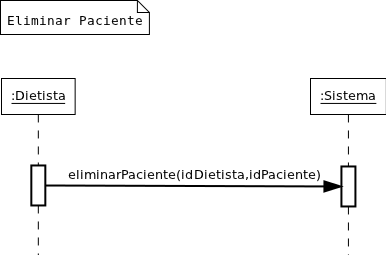
\includegraphics[scale=0.7]{../img/DS_EliminarPaciente.png}
  \end{center}
  \caption{Diagrama de secuencia: Eliminar Paciente}
\end{figure}
\textbf{Contrato de la operación:} eliminarPaciente(idDietista,idPaciente)
\begin{itemize}
\item \textbf{Responsabilidades:} Eliminar el perfil de un paciente del dietista en el sistema.
\item \textbf{Referencias cruzadas:} Caso de uso ``Eliminar Perfil Paciente''.
\item \textbf{Precondición:}
\begin{itemize}
\item El dietista con id = idDietista tiene su perfil abierto.
\item El paciente con id = idPaciente existe.
\end{itemize}
\item \textbf{Postcondición:}
\begin{itemize}
\item El paciente con idPaciente se elimina del sistema.
\end{itemize}
\end{itemize}

\textbf{Caso de Uso: Añadir Información Médica}
\begin{itemize}
\item \textbf{Descripción:} Añadir información médica a un paciente del sistema.
\item \textbf{Precondición:} El dietista y el paciente existen en el sistema.
\item \textbf{Postcondición:} Se añade la información médica al paciente del sistema.
\item \textbf{Actores:} Dietista(principal)
\item \textbf{Resumen:} El dietista desea añadir información médica a un paciente del sistema.
\item \textbf{Escenario Principal:}
\begin{enumerate}
\item El dietista solicita al sistema añadir información médica a un paciente.
\item El dietista introduce los campos solicitados.
\item El sistema almacena los datos en el sistema.
\end{enumerate}
\item \textbf{Escenario Alternativo:}
\begin{enumerate}
\item[0] En cualquier momento el dietista puede cancelar el proceso.
\end{enumerate}
\end{itemize}
\begin{figure}[H]
  \label{ds_anadirinfomed}
  \begin{center}
    % Comentar si no está el paquete tkiz instalado, y descomentar la
    % linea siguiente. Comentar además la inclusión del paquete en
    % estilos/estiloBase.sty
    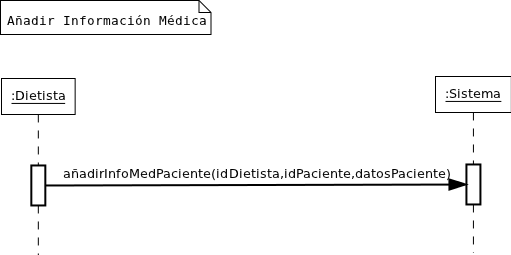
\includegraphics[scale=0.7]{../img/DS_AnadirInfoMed.png}
  \end{center}
  \caption{Diagrama de secuencia: Añadir Información Médica}
\end{figure}
\textbf{Contrato de la operación:} añadirInfoMedPaciente(idDietista,idPaciente,datosPaciente)
\begin{itemize}
\item \textbf{Responsabilidades:} Añadir información médica a un paciente del dietista en el sistema.
\item \textbf{Referencias cruzadas:} Caso de uso ``Añadir Información Médica''.
\item \textbf{Precondición:}
\begin{itemize}
\item El dietista con id = idDietista tiene su perfil abierto.
\item El paciente con id = idPaciente tiene su perfil abierto.
\item datosPaciente es válido.
\end{itemize}
\item \textbf{Postcondición:}
\begin{itemize}
\item Se añade la información médica al paciente en el sistema.
\end{itemize}
\end{itemize}

\textbf{Caso de Uso: Modificar Información Médica}
\begin{itemize}
\item \textbf{Descripción:} Modificar la información médica de un paciente del sistema.
\item \textbf{Precondición:} El dietista y el paciente existen en el sistema.
\item \textbf{Postcondición:} Se modifica la información médica al paciente del sistema.
\item \textbf{Actores:} Dietista(principal)
\item \textbf{Resumen:} El dietista desea modificar la información médica de un paciente del sistema.
\item \textbf{Escenario Principal:}
\begin{enumerate}
\item El dietista solicita al sistema modificar la información médica de un paciente.
\item El dietista introduce los campos solicitados.
\item El sistema almacena los datos en el sistema.
\end{enumerate}
\item \textbf{Escenario Alternativo:}
\begin{enumerate}
\item[0] En cualquier momento el dietista puede cancelar el proceso.
\end{enumerate}
\end{itemize}
\begin{figure}[H]
  \label{ds_modificarinfomed}
  \begin{center}
    % Comentar si no está el paquete tkiz instalado, y descomentar la
    % linea siguiente. Comentar además la inclusión del paquete en
    % estilos/estiloBase.sty
    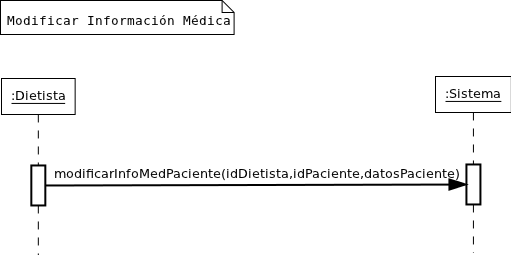
\includegraphics[scale=0.7]{../img/DS_ModificarInfoMed.png}
  \end{center}
  \caption{Diagrama de secuencia: Modificar Información Médica}
\end{figure}
\textbf{Contrato de la operación:} modificarInfoMedPaciente(idDietista,idPaciente,datosPaciente)
\begin{itemize}
\item \textbf{Responsabilidades:} Modificar información médica de un paciente del dietista en el sistema.
\item \textbf{Referencias cruzadas:} Caso de uso ``Modificar Información Médica''.
\item \textbf{Precondición:}
\begin{itemize}
\item El dietista con id = idDietista tiene su perfil abierto.
\item El paciente con id = idPaciente tiene su perfil abierto.
\item datosPaciente es válido.
\end{itemize}
\item \textbf{Postcondición:}
\begin{itemize}
\item Se modifica la información médica del paciente en el sistema.
\end{itemize}
\end{itemize}


\textbf{Caso de Uso: Añadir Información General}
\begin{itemize}
\item \textbf{Descripción:} Añadir información general a un paciente del sistema.
\item \textbf{Precondición:} El dietista y el paciente existen en el sistema.
\item \textbf{Postcondición:} Se añade la información general del paciente del sistema.
\item \textbf{Actores:} Dietista(principal) y Paciente(secundario)
\item \textbf{Resumen:} El dietista desea añadir información general a un paciente del sistema.
\item \textbf{Escenario Principal:}
\begin{enumerate}
\item El dietista solicita al sistema añadir información general a un paciente.
\item El dietista introduce los campos solicitados.
\item El sistema almacena los datos en el sistema.
\end{enumerate}
\item \textbf{Escenario Alternativo:}
\begin{enumerate}
\item[0] En cualquier momento el dietista puede cancelar el proceso.
\end{enumerate}
\end{itemize}
\begin{figure}[H]
  \label{ds_anadirinfogen}
  \begin{center}
    % Comentar si no está el paquete tkiz instalado, y descomentar la
    % linea siguiente. Comentar además la inclusión del paquete en
    % estilos/estiloBase.sty
    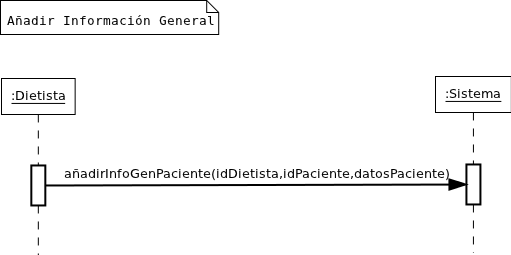
\includegraphics[scale=0.7]{../img/DS_AnadirInfoGen.png}
  \end{center}
  \caption{Diagrama de secuencia: Añadir Información General}
\end{figure}
\textbf{Contrato de la operación:} añadirInfoGenPaciente(idDietista,idPaciente,datosPaciente)
\begin{itemize}
\item \textbf{Responsabilidades:} Añadir información general a un paciente del dietista en el sistema.
\item \textbf{Referencias cruzadas:} Caso de uso ``Añadir Información General''.
\item \textbf{Precondición:}
\begin{itemize}
\item El dietista con id = idDietista tiene su perfil abierto.
\item El paciente con id = idPaciente tiene su perfil abierto.
\item datosPaciente es válido.
\end{itemize}
\item \textbf{Postcondición:}
\begin{itemize}
\item Se añade la información general al paciente en el sistema.
\end{itemize}
\end{itemize}

\textbf{Caso de Uso: Añadir Diario Dietético}
\begin{itemize}
\item \textbf{Descripción:} Añadir un diario dietético a un paciente del sistema.
\item \textbf{Precondición:} El dietista y el paciente existen en el sistema.
\item \textbf{Postcondición:} Se añade el diario dietético al paciente del sistema.
\item \textbf{Actores:} Dietista(principal) y Paciente(secundario)
\item \textbf{Resumen:} El dietista desea añadir un diario dietético a un paciente del sistema.
\item \textbf{Escenario Principal:}
\begin{enumerate}
\item El dietista solicita al sistema añadir un diario dietético a un paciente.
\item El dietista introduce los campos solicitados.
\item El sistema almacena los datos en el sistema.
\end{enumerate}
\item \textbf{Escenario Alternativo:}
\begin{enumerate}
\item[0] En cualquier momento el dietista puede cancelar el proceso.
\end{enumerate}
\end{itemize}
\begin{figure}[H]
  \label{ds_anadirdiariodiet}
  \begin{center}
    % Comentar si no está el paquete tkiz instalado, y descomentar la
    % linea siguiente. Comentar además la inclusión del paquete en
    % estilos/estiloBase.sty
    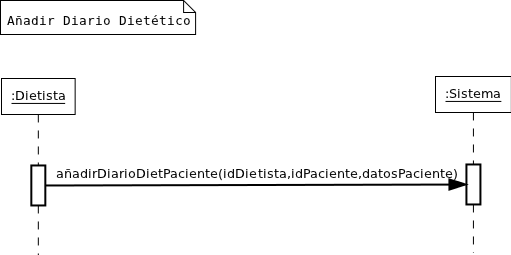
\includegraphics[scale=0.7]{../img/DS_AnadirDiarioDiet.png}
  \end{center}
  \caption{Diagrama de secuencia: Añadir Diario Dietético}
\end{figure}
\textbf{Contrato de la operación:} añadirDiarioDietPaciente(idDietista,idPaciente,datosPaciente)
\begin{itemize}
\item \textbf{Responsabilidades:} Añadir un diario dietético a un paciente del dietista en el sistema.
\item \textbf{Referencias cruzadas:} Caso de uso ``Añadir Diario Dietético''.
\item \textbf{Precondición:}
\begin{itemize}
\item El dietista con id = idDietista tiene su perfil abierto.
\item El paciente con id = idPaciente tiene su perfil abierto.
\item datosPaciente es válido.
\end{itemize}
\item \textbf{Postcondición:}
\begin{itemize}
\item Se añade el diario dietético al paciente en el sistema.
\end{itemize}
\end{itemize}


\textbf{Caso de Uso: Eliminar Diario Dietético}
\begin{itemize}
\item \textbf{Descripción:} Eliminar un diario dietético de un paciente del sistema.
\item \textbf{Precondición:} El dietista y el paciente existen en el sistema.
\item \textbf{Postcondición:} Se elimina el diario dietético del paciente del sistema.
\item \textbf{Actores:} Dietista(principal)
\item \textbf{Resumen:} El dietista desea eliminar un diario dietético de un paciente del sistema.
\item \textbf{Escenario Principal:}
\begin{enumerate}
\item El dietista solicita al sistema eliminar un diario dietético de un paciente.
\item El dietista selecciona el diario dietético a eliminar.
\item El sistema elimina el diario dietético del sistema.
\end{enumerate}
\item \textbf{Escenario Alternativo:}
\begin{enumerate}
\item[0] En cualquier momento el dietista puede cancelar el proceso.
\end{enumerate}
\end{itemize}
\begin{figure}[H]
  \label{ds_eliminardiariodiet}
  \begin{center}
    % Comentar si no está el paquete tkiz instalado, y descomentar la
    % linea siguiente. Comentar además la inclusión del paquete en
    % estilos/estiloBase.sty
    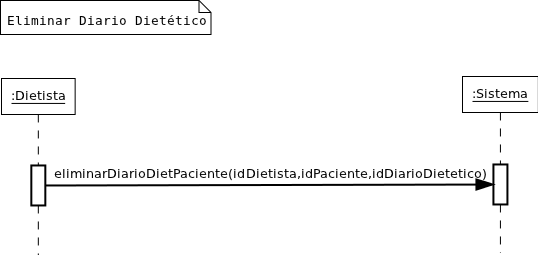
\includegraphics[scale=0.7]{../img/DS_EliminarDiarioDiet.png}
  \end{center}
  \caption{Diagrama de secuencia: Eliminar Diario Dietético}
\end{figure}
\textbf{Contrato de la operación:} eliminarDiarioDietPaciente(idDietista,idPaciente,idDiarioDietetico)
\begin{itemize}
\item \textbf{Responsabilidades:} Eliminar un diario dietético de un paciente del dietista en el sistema.
\item \textbf{Referencias cruzadas:} Caso de uso ``Eliminar Diario Dietético''.
\item \textbf{Precondición:}
\begin{itemize}
\item El dietista con id = idDietista tiene su perfil abierto.
\item El paciente con id = idPaciente tiene su perfil abierto.
\item Existe un diario dietético con id = idDiarioDietetico.
\end{itemize}
\item \textbf{Postcondición:}
\begin{itemize}
\item Se elimina el diario dietético del paciente en el sistema.
\end{itemize}
\end{itemize}


\textbf{Caso de Uso: Añadir Recordatorio}
\begin{itemize}
\item \textbf{Descripción:} Añadir un recordatorio 24h a un paciente del sistema.
\item \textbf{Precondición:} El dietista y el paciente existen en el sistema.
\item \textbf{Postcondición:} Se añade el recordatorio 24h al paciente del sistema.
\item \textbf{Actores:} Dietista(principal) y Paciente(secundario)
\item \textbf{Resumen:} El dietista desea añadir un recordatorio 24h a un paciente del sistema.
\item \textbf{Escenario Principal:}
\begin{enumerate}
\item El dietista solicita al sistema añadir un recordatorio 24h a un paciente.
\item El dietista introduce los campos solicitados.
\item El sistema almacena los datos en el sistema.
\end{enumerate}
\item \textbf{Escenario Alternativo:}
\begin{enumerate}
\item[0] En cualquier momento el dietista puede cancelar el proceso.
\end{enumerate}
\end{itemize}
\begin{figure}[H]
  \label{ds_anadirrecordatorio}
  \begin{center}
    % Comentar si no está el paquete tkiz instalado, y descomentar la
    % linea siguiente. Comentar además la inclusión del paquete en
    % estilos/estiloBase.sty
    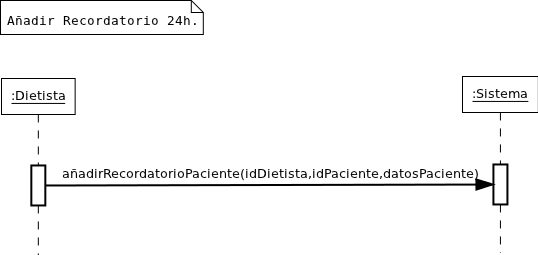
\includegraphics[scale=0.7]{../img/DS_AnadirRecordatorio.png}
  \end{center}
  \caption{Diagrama de secuencia: Añadir Recordatorio 24h}
\end{figure}
\textbf{Contrato de la operación:} añadirRecordatorioPaciente(idDietista,idPaciente,datosPaciente)
\begin{itemize}
\item \textbf{Responsabilidades:} Añadir un recordatorio 24h a un paciente del dietista en el sistema.
\item \textbf{Referencias cruzadas:} Caso de uso ``Añadir Recordatorio''.
\item \textbf{Precondición:}
\begin{itemize}
\item El dietista con id = idDietista tiene su perfil abierto.
\item El paciente con id = idPaciente tiene su perfil abierto.
\item datosPaciente es válido.
\end{itemize}
\item \textbf{Postcondición:}
\begin{itemize}
\item Se añade el recordatorio 24h al paciente en el sistema.
\end{itemize}
\end{itemize}


\textbf{Caso de Uso: Eliminar Recordatorio}
\begin{itemize}
\item \textbf{Descripción:} Eliminar un recordatorio 24h de un paciente del sistema.
\item \textbf{Precondición:} El dietista y el paciente existen en el sistema.
\item \textbf{Postcondición:} Se elimina el recordatorio 24h del paciente del sistema.
\item \textbf{Actores:} Dietista(principal)
\item \textbf{Resumen:} El dietista desea eliminar un recordatorio 24h de un paciente del sistema.
\item \textbf{Escenario Principal:}
\begin{enumerate}
\item El dietista solicita al sistema eliminar un recordatorio 24h de un paciente.
\item El dietista selecciona el recordatorio 24h a eliminar.
\item El sistema elimina el recordatorio 24h del sistema.
\end{enumerate}
\item \textbf{Escenario Alternativo:}
\begin{enumerate}
\item[0] En cualquier momento el dietista puede cancelar el proceso.
\end{enumerate}
\end{itemize}
\begin{figure}[H]
  \label{ds_eliminarrecordatorio}
  \begin{center}
    % Comentar si no está el paquete tkiz instalado, y descomentar la
    % linea siguiente. Comentar además la inclusión del paquete en
    % estilos/estiloBase.sty
    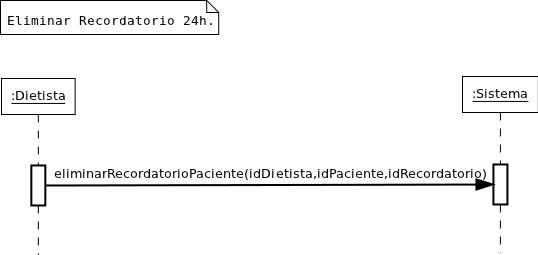
\includegraphics[scale=0.7]{../img/DS_EliminarRecordatorio.png}
  \end{center}
  \caption{Diagrama de secuencia: Eliminar Recordatorio 24h.}
\end{figure}
\textbf{Contrato de la operación:} eliminarRecordatorioPaciente(idDietista,idPaciente,idRecordatorio)
\begin{itemize}
\item \textbf{Responsabilidades:} Eliminar un recordatorio 24h de un paciente del dietista en el sistema.
\item \textbf{Referencias cruzadas:} Caso de uso ``Eliminar Recordatorio''.
\item \textbf{Precondición:}
\begin{itemize}
\item El dietista con id = idDietista tiene su perfil abierto.
\item El paciente con id = idPaciente tiene su perfil abierto.
\item Existe un recordatorio 24h con id = idRecordatorio.
\end{itemize}
\item \textbf{Postcondición:}
\begin{itemize}
\item Se elimina el recordatorio 24h del paciente en el sistema.
\end{itemize}
\end{itemize}

\textbf{Caso de Uso: Añadir Frecuencia de Ingesta}
\begin{itemize}
\item \textbf{Descripción:} Añadir la frecuencia de ingesta de alimentos de un paciente del sistema.
\item \textbf{Precondición:} El dietista y el paciente existen en el sistema.
\item \textbf{Postcondición:} Se añade la frecuencia de ingesta de alimentos al paciente del sistema.
\item \textbf{Actores:} Dietista(principal) y Paciente(secundario)
\item \textbf{Resumen:} El dietista desea añadir la frecuencia de ingesta de alimentos a un paciente del sistema.
\item \textbf{Escenario Principal:}
\begin{enumerate}
\item El dietista solicita al sistema añadir la frecuencia de ingesta de alimentos a un paciente.
\item El dietista introduce los campos solicitados.
\item El sistema almacena los datos en el sistema.
\end{enumerate}
\item \textbf{Escenario Alternativo:}
\begin{enumerate}
\item[0] En cualquier momento el dietista puede cancelar el proceso.
\end{enumerate}
\end{itemize}
\begin{figure}[H]
  \label{ds_anadirfrecing}
  \begin{center}
    % Comentar si no está el paquete tkiz instalado, y descomentar la
    % linea siguiente. Comentar además la inclusión del paquete en
    % estilos/estiloBase.sty
    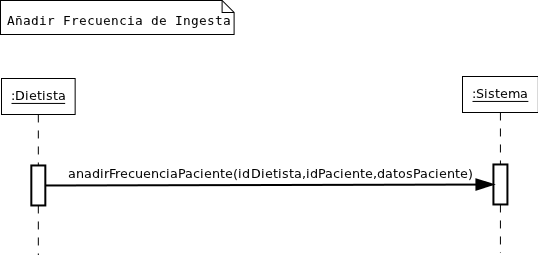
\includegraphics[scale=0.7]{../img/DS_AnadirFrecIng.png}
  \end{center}
  \caption{Diagrama de secuencia: Añadir Frecuencia de Ingesta}
\end{figure}
\textbf{Contrato de la operación:} añadirFrecuenciaPaciente(idDietista,idPaciente,datosPaciente)
\begin{itemize}
\item \textbf{Responsabilidades:} Añadir la frecuencia de ingesta de alimentos a un paciente del dietista en el sistema.
\item \textbf{Referencias cruzadas:} Caso de uso ``Añadir Frecuencia de Ingesta''.
\item \textbf{Precondición:}
\begin{itemize}
\item El dietista con id = idDietista tiene su perfil abierto.
\item El paciente con id = idPaciente tiene su perfil abierto.
\item datosPaciente es válido.
\end{itemize}
\item \textbf{Postcondición:}
\begin{itemize}
\item Se añade la frecuencia de ingesta de alimentos al paciente en el sistema.
\end{itemize}
\end{itemize}


\textbf{Caso de Uso: Añadir Recetas a Semanario}
\begin{itemize}
\item \textbf{Descripción:} Añadir una receta al semanario de un paciente del sistema.
\item \textbf{Precondición:} El dietista y el paciente existen en el sistema.
\item \textbf{Postcondición:} Se añade una receta al semanario del paciente del sistema.
\item \textbf{Actores:} Dietista(principal)
\item \textbf{Resumen:} El dietista desea añadir una receta al semanario de un paciente del sistema.
\item \textbf{Escenario Principal:}
\begin{enumerate}
\item El dietista solicita al sistema añadir una receta al semanario de un paciente.
\item El dietista selecciona la receta a añadir.
\item El sistema registra los datos en el sistema.
\end{enumerate}
\item \textbf{Escenario Alternativo:}
\begin{enumerate}
\item[0] En cualquier momento el dietista puede cancelar el proceso.
\end{enumerate}
\end{itemize}
\begin{figure}[H]
  \label{ds_anadirrecetasemanario}
  \begin{center}
    % Comentar si no está el paquete tkiz instalado, y descomentar la
    % linea siguiente. Comentar además la inclusión del paquete en
    % estilos/estiloBase.sty
    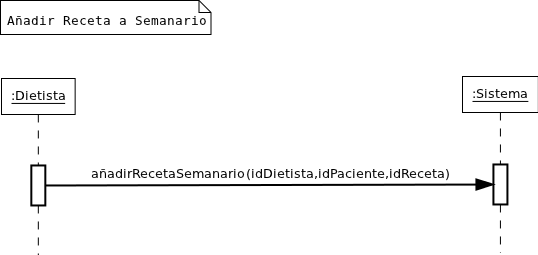
\includegraphics[scale=0.7]{../img/DS_AnadirRecetaSemanario.png}
  \end{center}
  \caption{Diagrama de secuencia: Añadir Receta a Semanario}
\end{figure}
\textbf{Contrato de la operación:} añadirRecetaSemanario(idDietista,idPaciente,idReceta)
\begin{itemize}
\item \textbf{Responsabilidades:} Añadir una receta al semanario de un paciente del dietista en el sistema.
\item \textbf{Referencias cruzadas:} Caso de uso ``Añadir Receta a Semanario''.
\item \textbf{Precondición:}
\begin{itemize}
\item El dietista con id = idDietista tiene su perfil abierto.
\item El paciente con id = idPaciente tiene su perfil abierto.
\item Existe una receta con id = idReceta.
\end{itemize}
\item \textbf{Postcondición:}
\begin{itemize}
\item Se añade la receta al semanario del paciente en el sistema.
\end{itemize}
\end{itemize}


\textbf{Caso de Uso: Ver Semanarios}
\begin{itemize}
\item \textbf{Descripción:} Ver semanarios de un paciente del sistema.
\item \textbf{Precondición:} El dietista y el paciente existen en el sistema.
\item \textbf{Postcondición:} Ninguna.
\item \textbf{Actores:} Dietista(principal)
\item \textbf{Resumen:} El dietista desea ver los semanarios de un paciente del sistema.
\item \textbf{Escenario Principal:}
\begin{enumerate}
\item El dietista solicita al sistema ver los semanarios de un paciente.
\item El sistema muestra los datos en el sistema.
\end{enumerate}
\item \textbf{Escenario Alternativo:}
\begin{enumerate}
\item[0] En cualquier momento el dietista puede cancelar el proceso.
\item[2] No hay ningún semanario registrado del paciente. El sistema no mostrará nada.
\end{enumerate}
\end{itemize}
\begin{figure}[H]
  \label{ds_versemanarios}
  \begin{center}
    % Comentar si no está el paquete tkiz instalado, y descomentar la
    % linea siguiente. Comentar además la inclusión del paquete en
    % estilos/estiloBase.sty
    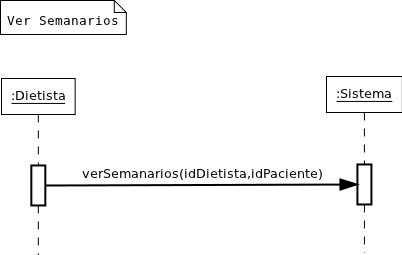
\includegraphics[scale=0.7]{../img/DS_VerSemanarios.png}
  \end{center}
  \caption{Diagrama de secuencia: Ver Semanarios de un Paciente}
\end{figure}
\textbf{Contrato de la operación:} verSemanarios(idDietista,idPaciente)
\begin{itemize}
\item \textbf{Responsabilidades:} Ver los semanarios de un paciente del dietista en el sistema.
\item \textbf{Referencias cruzadas:} Caso de uso ``Ver Semanarios''.
\item \textbf{Precondición:}
\begin{itemize}
\item El dietista con id = idDietista tiene su perfil abierto.
\item El paciente con id = idPaciente tiene su perfil abierto.
\end{itemize}
\item \textbf{Postcondición:}
\begin{itemize}
\item El sistema muestra los semanarios del paciente del sistema.
\end{itemize}
\end{itemize}

\newpage
\subsubsection{Casos de uso respecto a la gestión de recetas}

\begin{figure}[H]
  \label{cu_receta}
  \begin{center}
    % Comentar si no está el paquete tkiz instalado, y descomentar la
    % linea siguiente. Comentar además la inclusión del paquete en
    % estilos/estiloBase.sty
    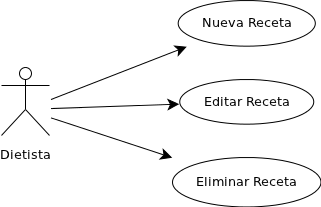
\includegraphics[scale=0.5]{../img/CU_Receta.png}
  \end{center}
  \caption{Diagrama de caso de uso: Gestión de recetas}
\end{figure}

\textbf{Caso de Uso: Nueva Receta}
\begin{itemize}
\item \textbf{Descripción:} Añadir una nueva receta en el sistema.
\item \textbf{Precondición:} Hay un dietista en uso y la receta no existe.
\item \textbf{Postcondición:} La receta del dietista se registra en el sistema.
\item \textbf{Actores:} Dietista(principal)
\item \textbf{Resumen:} El dietista desea registrar una nueva receta en el sistema.
\item \textbf{Escenario Principal:}
\begin{enumerate}
\item El dietista solicita al sistema registrar una nueva receta.
\item El dietista rellena los campos solicitados para la receta.
\item El sistema comprueba los datos.
\item El sistema almacena los datos.
\end{enumerate}
\item \textbf{Escenario Alternativo:}
\begin{enumerate}
\item[0] El dietista puede cancelar el proceso en cualquier momento.
\item[3] La receta ya existe en el sistema. Mensaje de advertencia del sistema.
\end{enumerate}
\end{itemize}
\begin{figure}[H]
  \label{ds_nuevareceta}
  \begin{center}
    % Comentar si no está el paquete tkiz instalado, y descomentar la
    % linea siguiente. Comentar además la inclusión del paquete en
    % estilos/estiloBase.sty
    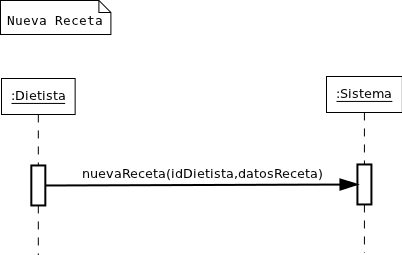
\includegraphics[scale=0.7]{../img/DS_NuevaReceta.png}
  \end{center}
  \caption{Diagrama de secuencia: Nueva Receta}
\end{figure}
\textbf{Contrato de la operación:} nuevaReceta(idDietista, datosReceta)
\begin{itemize}
\item \textbf{Responsabilidades:} Registrar una nueva receta en el sistema.
\item \textbf{Referencias cruzadas:} Caso de uso ``Nueva Receta''.
\item \textbf{Precondición:}
\begin{itemize}
\item Existe un dietista con id = idDietista en uso.
\item datosReceta es válido.
\end{itemize}
\item \textbf{Postcondición:}
\begin{itemize}
\item La receta se guarda en el sistema.
\end{itemize}
\end{itemize}

\textbf{Caso de Uso: Editar Receta}
\begin{itemize}
\item \textbf{Descripción:} Editar una receta del sistema.
\item \textbf{Precondición:} Hay un dietista en uso y la receta existe.
\item \textbf{Postcondición:} La receta del dietista se registra en el sistema con los nuevos datos.
\item \textbf{Actores:} Dietista(principal)
\item \textbf{Resumen:} El dietista desea editar una receta del sistema.
\item \textbf{Escenario Principal:}
\begin{enumerate}
\item El dietista solicita al sistema editar una receta.
\item El sistema muestra el listado de recetas.
\item El dietista selecciona la receta a editar.
\item El dietista rellena los campos que desea cambiar para la receta.
\item El sistema almacena los nuevos datos.
\end{enumerate}
\item \textbf{Escenario Alternativo:}
\begin{enumerate}
\item[0] El dietista puede cancelar el proceso en cualquier momento.
\end{enumerate}
\end{itemize}
\begin{figure}[H]
  \label{ds_editarreceta}
  \begin{center}
    % Comentar si no está el paquete tkiz instalado, y descomentar la
    % linea siguiente. Comentar además la inclusión del paquete en
    % estilos/estiloBase.sty
    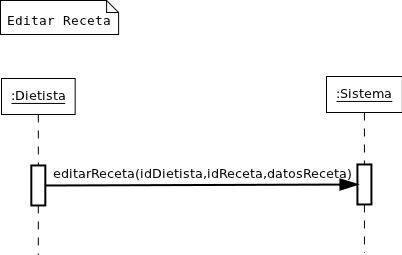
\includegraphics[scale=0.7]{../img/DS_EditarReceta.png}
  \end{center}
  \caption{Diagrama de secuencia: Editar Receta}
\end{figure}
\textbf{Contrato de la operación:} editarReceta(idDietista, idReceta, datosReceta)
\begin{itemize}
\item \textbf{Responsabilidades:} Editar una receta del sistema.
\item \textbf{Referencias cruzadas:} Caso de uso ``Editar Receta''.
\item \textbf{Precondición:}
\begin{itemize}
\item Existe un dietista con id = idDietista en uso.
\item Existe una receta con id = idReceta.
\item datosReceta es válido.
\end{itemize}
\item \textbf{Postcondición:}
\begin{itemize}
\item La receta se guarda con los nuevos datos en el sistema.
\end{itemize}
\end{itemize}

\textbf{Caso de Uso: Eliminar Receta}
\begin{itemize}
\item \textbf{Descripción:} Eliminar una receta del sistema.
\item \textbf{Precondición:} Hay un dietista en uso y la receta existe.
\item \textbf{Postcondición:} La receta del dietista se elimina del sistema.
\item \textbf{Actores:} Dietista(principal)
\item \textbf{Resumen:} El dietista desea eliminar una receta del sistema.
\item \textbf{Escenario Principal:}
\begin{enumerate}
\item El dietista solicita al sistema eliminar una receta.
\item El sistema muestra el listado de recetas.
\item El dietista selecciona la receta a eliminar.
\item El sistema elimina la receta del sistema.
\end{enumerate}
\item \textbf{Escenario Alternativo:}
\begin{enumerate}
\item[0] El dietista puede cancelar el proceso en cualquier momento.
\end{enumerate}
\end{itemize}
\begin{figure}[H]
  \label{ds_eliminarreceta}
  \begin{center}
    % Comentar si no está el paquete tkiz instalado, y descomentar la
    % linea siguiente. Comentar además la inclusión del paquete en
    % estilos/estiloBase.sty
    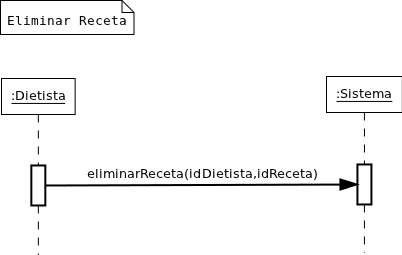
\includegraphics[scale=0.7]{../img/DS_EliminarReceta.png}
  \end{center}
  \caption{Diagrama de secuencia: Eliminar Receta}
\end{figure}
\textbf{Contrato de la operación:} eliminarReceta(idDietista, idReceta)
\begin{itemize}
\item \textbf{Responsabilidades:} Eliminar una receta del sistema.
\item \textbf{Referencias cruzadas:} Caso de uso ``Eliminar Receta''.
\item \textbf{Precondición:}
\begin{itemize}
\item Existe un dietista con id = idDietista en uso.
\item Existe una receta con id = idReceta.
\end{itemize}
\item \textbf{Postcondición:}
\begin{itemize}
\item La receta se elimina del sistema.
\end{itemize}
\end{itemize}

\subsection{Modelos conceptual de datos.}
\subsubsection{Diagrama conceptual de clases.}
\begin{figure}[H]
  \label{ds_eliminarreceta}
  \begin{center}
    % Comentar si no está el paquete tkiz instalado, y descomentar la
    % linea siguiente. Comentar además la inclusión del paquete en
    % estilos/estiloBase.sty
    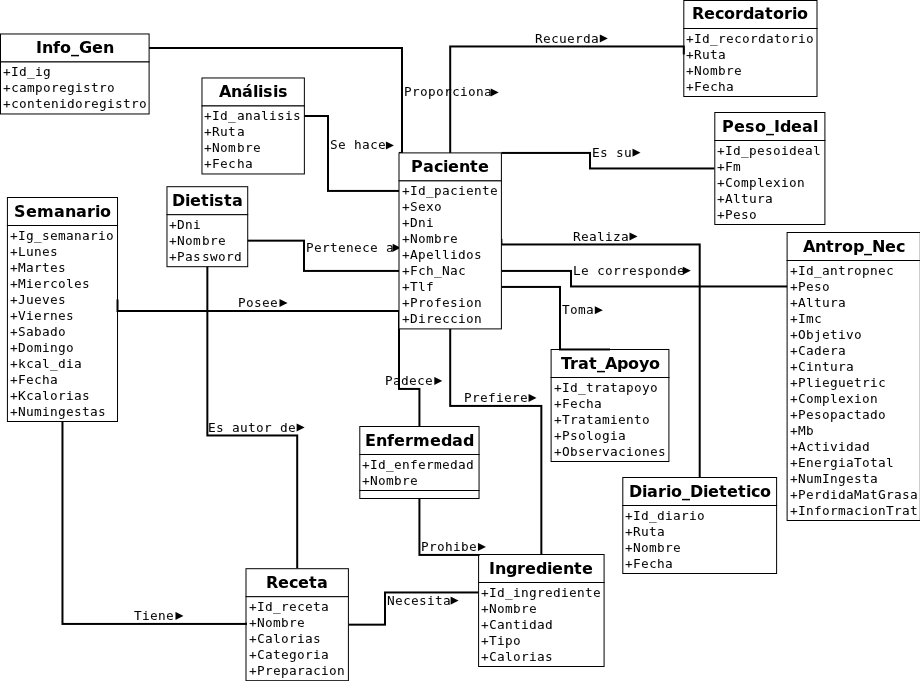
\includegraphics[scale=0.5]{../img/Diagrama_Clases.png}
  \end{center}
  \caption{Modelo conceptual de datos: Diagrama conceptual de clases}
\end{figure}
\subsubsection{Restricciones de clave primaria.}
\textbf{Clave primaria:}
(Dietista, d\_dni),
(Paciente, p\_id),
(Semanario, s\_id),
(Enfermedad, ep\_id),
(Receta, r\_id),
(Ingrediente, i\_id)


\chapter{Diseño del Sistema}
% ------------------------------------------------------------------------------
% Este fichero es parte de la plantilla LaTeX para la realización de Proyectos
% Final de Grado, protegido bajo los términos de la licencia GFDL.
% Para más información, la licencia completa viene incluida en el
% fichero fdl-1.3.tex

% Copyright (C) 2012 SPI-FM. Universidad de Cádiz
% ------------------------------------------------------------------------------

Para el diseño del sistema se ha optado por el patrón arquitectónico en tres capas. Éste divide el trabajo en tres niveles, repartiendo claramente las funciones.\\
Las capas se detallan a continuación:
\begin{itemize}
\item \textbf{Capa de presentación}: encargada de interactuar con el usuario.
\item \textbf{Capa de dominio}: encargada de implementar las funcionalidades del sistema.
\item \textbf{Capa de gestión de datos}: encargada de interactuar con el ``Sistema de Gestión de la Base de Datos (\textit{SGBD})''.
\end{itemize}
Las capas estan ordenadas de mayor a menor nivel de abstracción. Dichas capas se comunican con su capa contigua.\\

\section{Diseño de la capa de gestión de datos}
\subsection{Invocación de consultas SQL}
Las consultas SQL las realizan las clases declaradas en los archivos  principales ``.py'' de la aplicación.\\
\begin{itemize}
\item \textbf{La clase ``Dietista''}:
\begin{itemize}
\item \textbf{Método ``Verificar''}: realiza una consulta para verificar que un nuevo dietista no existe en el sistema.
\item \textbf{Método ``GuardarDietista''}: realiza una consulta para guardar los datos de un nuevo dietista en el sistema.
\item \textbf{Método ``MostrarDietistas''}: realiza una consulta para mostrar dietistas existentes en el sistema.
\item \textbf{Método ``Aceptar''}: realiza una consulta para verificar la contraseña de un dietista para su logueo en el sistema.
\item \textbf{Método ``ElimPerf''}: realiza una consulta para eliminar un dietista existente.
\end{itemize}
\item \textbf{La clase ``Paciente''}:
\begin{itemize}
\item \textbf{Método ``MostrarVentana2NPaciente''}: realiza una consulta para asignar un nuevo id al paciente nuevo.
\item \textbf{Método ``GuardarPaciente''}: realiza una consulta para guardar los datos de un paciente nuevo.
\item \textbf{Método ``AbrirPaciente''}: realiza una consulta para seleccionar los datos de un paciente existente.
\item \textbf{Método ``MostrarDatosP''}: realiza una consulta para mostrar todos los datos relacionados de un paciente existente.
\item \textbf{Método ``EliminarPaciente''}: realiza una consulta para tomar los datos del paciente a eliminar.
\item \textbf{Método ``DropPaciente''}: realiza una consulta para eliminar todos los datos relacionados del paciente.
\item \textbf{Método ``MostrarAnalisis''}: realiza una consulta para mostrar los análisis de un paciente.
\item \textbf{Método ``MostrarEnfPaciente''}: realiza una consulta para mostrar las enfermedades y patologías de un paciente.
\item \textbf{Método ``abrirDialogo''}: realiza una consulta para insertar un análisis a través de un diálogo de selección.
\item \textbf{Método ``EliminarAnalitica''}: realiza una consulta para eliminar una análisis.
\item \textbf{Método ``VerAnalitica''}: realiza una consulta para abrir el análisis.
\item \textbf{Método ``GuardarTrat''}: realiza una consulta para guardar el tratamiento farmacológico de un paciente.
\item \textbf{Método ``MostrarTratA''}: realiza una consulta para guardar el tratamiento de apoyo de un paciente.
\item \textbf{Método ``ElimItem''}: realiza una consulta para eliminar un tratamiento de apoyo de un paciente.
\item \textbf{Método ``ElimEnfBBDD''}: realiza una consulta para eliminar una enfermedad del sistema.
\item \textbf{Método ``CrearEnfermedad''}: realiza una consulta para crear una enfermedad o patología en el sistema.
\item \textbf{Método ``AnadirEnfermedad''}: realiza una consulta para añadir una enfermedad a un paciente.
\item \textbf{Método ``EliminarEP''}: realiza una consulta para eliminar una enfermedad del sistema.
\item \textbf{Método ``MostrarListadoEnf''}: realiza una consulta para mostrar el listado de enfermedades y patologías.
\item \textbf{Método ``ExcluirRecetasEnf''}: realiza una consulta para eliminar las recetas según los ingredientes que tenga la enfermedad.
\item \textbf{Método ``GuardarInfoG''}: realiza una consulta para guardar la información general de un paciente.
\item \textbf{Método ``MostrarInfoG''}: realiza una consulta para mostrar la información general de un paciente.
\item \textbf{Método ``MostrarDiario''}: realiza una consulta para mostrar los diarios dietéticos de un paciente.
\item \textbf{Método ``abrirDialogoD''}: realiza una consulta para añadir un diario dietético mediante un diálogo.
\item \textbf{Método ``EliminarDiario''}: realiza una consulta para eliminar un diario dietético seleccionado.
\item \textbf{Método ``VerDiario''}: realiza una consulta para abrir un diario dietético seleccionado.
\item \textbf{Método ``MostrarRecordatorio''}: realiza una consulta para mostrar los recordatorios 24h. existentes.
\item \textbf{Método ``abrirDialogoR''}: realiza una consulta para añadir un recordatorio 24h. mediante un diálogo.
\item \textbf{Método ``EliminarRecordatorio''}: realiza una consulta para eliminar un recordatorio 24h. seleccionado.
\item \textbf{Método ``VerRecordatorio''}: realiza una consulta para abrir un recordatorio 24h. seleccionado.
\item \textbf{Método ``MostrarPreferencias''}: realiza una consulta para iniciar la ventana de preferencias con los ingredientes existentes.
\item \textbf{Método ``AbrirCuestionarioFrec''}: realiza una consulta para abrir el cuestionario de frecuencia de un paciente.
\item \textbf{Método ``GuardarCuestionarioFrec''}: realiza una consulta para guardar el cuestionario de frecuencia del paciente.
\item \textbf{Método ``AccionGuardar''}: realiza una consulta para guardar los datos de un paciente.
\item \textbf{Método ``VerRecetas''}: realiza una consulta para mostrar los semanarios de un paciente.
\item \textbf{Método ``Ver''}: realiza una consulta para tomar los datos del semanario seleccionado.
\item \textbf{Método ``Utilizar''}: realiza una consulta para utilizar los datos en el semanario actual del semanario seleccionado. 
\item \textbf{Método ``Imprimir''}: realiza una consulta para tomar los datos a imprimir.
\end{itemize}
\item \textbf{La clase ``Receta''}:
\begin{itemize}
\item \textbf{Método ``MostrarIngred''}: realiza una consulta para mostrar todos los ingredientes existentes.
\item \textbf{Método ``AgregarIngr''}: realiza una consulta para agregar el ingrediente a la receta.
\item \textbf{Método ``ModificarIngr''}: realiza una consulta para modificar los datos de un ingrediente en la receta a modificar. 
\item \textbf{Método ``GuardarReceta''}: realiza una consulta para guardar los datos de la receta en el sistema.
\item \textbf{Método ``MostrarRecetas''}: realiza una consulta para mostrar la lista de recetas existentes.
\item \textbf{Método ``SeleccionarReceta''}: realiza una consulta para tomar los datos de una receta seleccionada.
\item \textbf{Método ``listElimReceta''}: realiza una consulta para mostrar las recetas existentes a eliminar.
\item \textbf{Método ``DropReceta''}: realiza una consulta para eliminar una receta.
\item \textbf{Método ``VentanaModificar''}: realiza una consulta para mostrar los datos de la receta a modificar.
\end{itemize}
\item \textbf{La clase ``Ingrediente''}:
\begin{itemize}
\item \textbf{Método ``GuardarIngrediente''}: realiza una consulta para guardar los datos de un ingrediente.
\item \textbf{Método ``ModificarIngrediente''}: realiza una consulta para modificar los datos de un ingrediente.
\item \textbf{Método ``RecogerPreferencias''}: realiza una consulta para mostrar las preferencias sobre el ingrediente.
\end{itemize}
\item \textbf{La clase ``Mainmenu''}:
\begin{itemize}
\item \textbf{Método ``mostrarPI''}: realiza una consulta para mostrar el peso ideal de un paciente.
\end{itemize}
\end{itemize}


\section{Diseño de la capa de dominio}
\subsection{Diagrama de interacción}
En este apartado se expondrán algunos de los diagramas de secuencia del diseño de la aplicación. Se utiliza un \textit{Patrón Controlador} en cada caso de uso descrito, es decir, una clase de control para llevar a cabo la operación solicitada.
\begin{itemize}
\item \textbf{Diagrama de secuencia para el caso de uso nuevo dietista}:
\begin{figure}[H]
  \label{ndiet}
  \begin{center}
    % Comentar si no está el paquete tkiz instalado, y descomentar la
    % linea siguiente. Comentar además la inclusión del paquete en
    % estilos/estiloBase.sty
    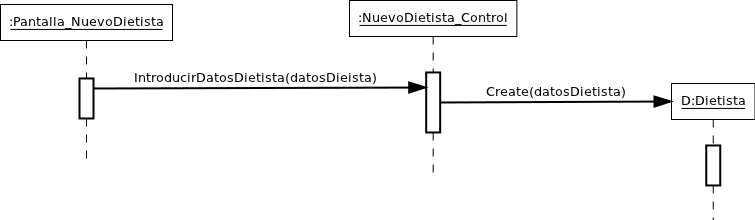
\includegraphics[scale=0.5]{../img/DI_NuevoDietista.png}
  \end{center}
  \caption{Diagrama de Interacción: Nuevo Dietista}
\end{figure}

\item \textbf{Diagrama de secuencia para el caso de uso nuevo paciente}: similar a aquellos casos de uso que suponen la creación de un objeto nuevo en la aplicación.
\begin{figure}[H]
  \label{npaciente}
  \begin{center}
    % Comentar si no está el paquete tkiz instalado, y descomentar la
    % linea siguiente. Comentar además la inclusión del paquete en
    % estilos/estiloBase.sty
    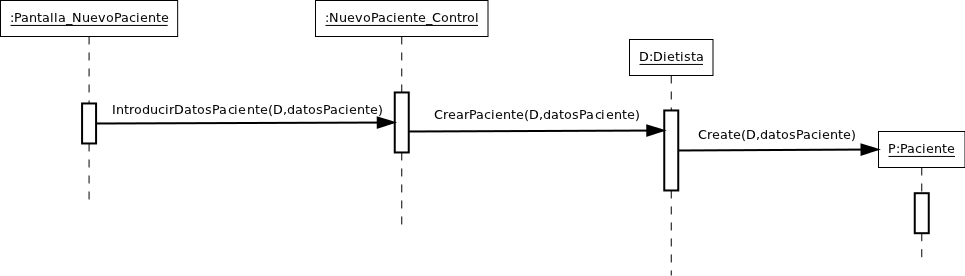
\includegraphics[scale=0.4]{../img/DI_NuevoPaciente.png}
  \end{center}
  \caption{Capa de presentación: Nuevo Paciente}
\end{figure}
\end{itemize}

A continuación se detallan los contratos de operaciones vistos en los diagramas de interacción.
\begin{itemize}
\item Nuevo Dietista:
\begin{itemize}
\item \textit{IntroducirDatosDietista(datosDietista)}: inicia la operación de introducción de los datos de un dietista en la aplicación.
\item \textit{Create(datosDietista)}: se crea un dietista con los datos especificados en datosDietista.
\end{itemize}
\item Nuevo Paciente:
\begin{itemize}
\item \textit{IntroducirDatosPaciente(D,datosPaciente)}: inicia la operación de introducción de los datos de un paciente en la aplicación.
\item \textit{CrearPaciente(D,datosPaciente)}: ordena al dietista D iniciar la creación de un paciente.
\item \textit{Create(D,datosPaciente)}: se crea un paciente con los datos especificados en datosPaciente.
\end{itemize}
\end{itemize}
\newpage


\section{Diseño de la capa de presentación}
Esta capa es la encargada de la interacción con el usuario, por lo que es importante que la primera impresión del usuario con respecto a la interfaz de la aplicación sea grata. La interfaz ha sido desarrollada bajo la biblioteca \textit{Qt}, así la apariencia visual de la misma se adaptará al tema de escritorio del usuario.\\
Se mostrarán a continuación algunos de los aspectos de la interfaz.
\begin{itemize}
\item \textbf{Menú principal}: ventana principal de la aplicación. Desde aquí el usuario podrá acceder a todas las funcionalidades del sistema. Se ha desarrollado buscando que la interfaz sea intuitiva, facilitando que el usuario encuentre rápidamente aquello que desee realizar. El menú principal constará de:
\begin{itemize}
\item \textbf{Barra de menú superior}: situado en la parte superior de la ventana, será la encargada de ofrecer las funcionalidades de los subsistemas de la aplicación. Cada botón tiene un nombre asociado referente a la tarea que realiza, facilitando así la interactuación del usuario.
\item \textbf{Área de información rápida}: situado inmediatamente debajo de la barra de menú superior, será donde el dietista podrá visualizar las referencias rápidas de ese paciente como recordatorio y orientación, facilitando así el trabajo.
\item \textbf{Pestañas interiores de información e interactuación}: a continuación nos encontramos con las pestañas de información e interactuación, desde las cuales el dietista podrá consultar y modificar los datos de un paciente, clasificados en pestañas que engloban información relacionada, haciendo más intuitivo el trabajo.
\begin{figure}[H]
  \label{ppral}
  \begin{center}
    % Comentar si no está el paquete tkiz instalado, y descomentar la
    % linea siguiente. Comentar además la inclusión del paquete en
    % estilos/estiloBase.sty
    \includegraphics[scale=0.5]{../../Image/aplicacion.png}
  \end{center}
  \caption{Capa de presentación: Menú Principal}
\end{figure}
\end{itemize}

\newpage
\item \textbf{Pestañas de información e interactuación:} constará de cuatro pestañas, desde las cuales se manejará la información relevante sobre el paciente.
\begin{itemize}
\item \textbf{Datos Personales}: ubicación de los datos personales más relevantes del paciente, a los que el dietista puede recurrir de un vistazo.\\\\
\begin{figure}[H]
  \label{datos}
  \begin{center}
    % Comentar si no está el paquete tkiz instalado, y descomentar la
    % linea siguiente. Comentar además la inclusión del paquete en
    % estilos/estiloBase.sty
    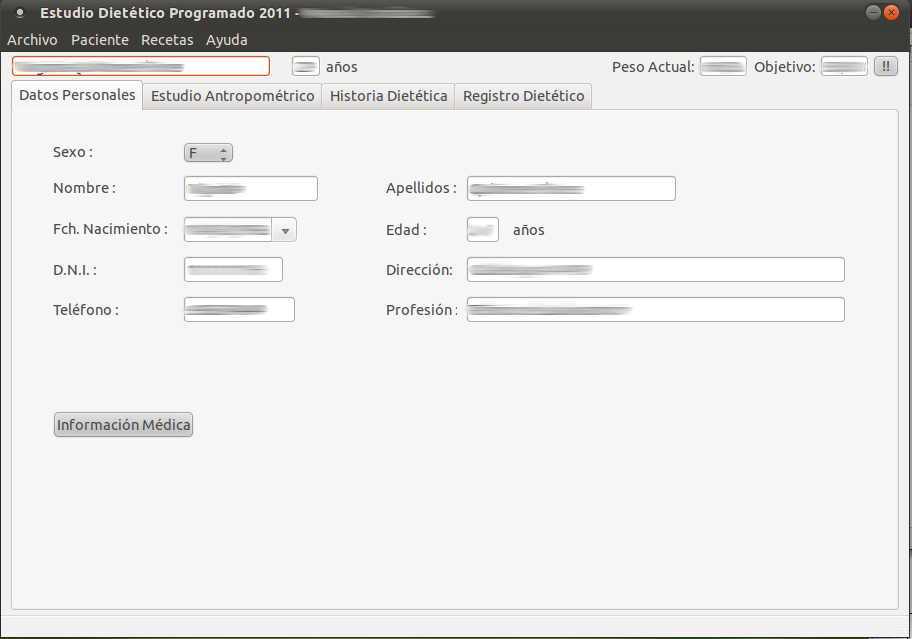
\includegraphics[scale=0.5]{../../Image/paciente-datos.png}
  \end{center}
  \caption{Capa de presentación: Pestaña Datos Personales}
\end{figure}
\newpage
\item \textbf{Estudio Antropométrico}: ubicación de los datos antropométricos del paciente, desde el cual se trabajará en mayor medida a lo largo del seguimiento del paciente.\\\\
\begin{figure}[H]
  \label{antrop}
  \begin{center}
    % Comentar si no está el paquete tkiz instalado, y descomentar la
    % linea siguiente. Comentar además la inclusión del paquete en
    % estilos/estiloBase.sty
    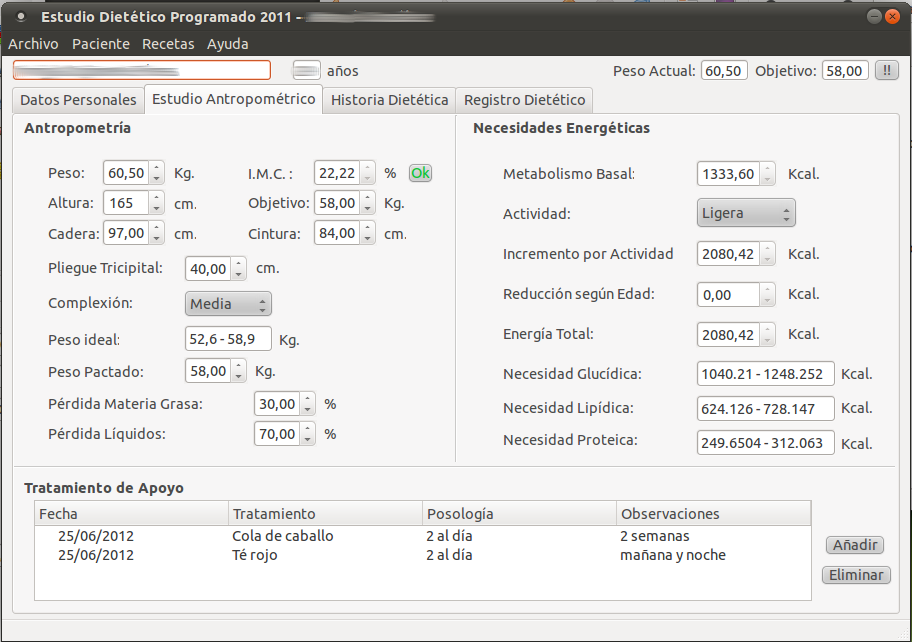
\includegraphics[scale=0.5]{../../Image/paciente-antrop.png}
  \end{center}
  \caption{Capa de presentación: Pestaña Estudio Antropométrico}
\end{figure}
\newpage
\item \textbf{Historia Dietética}: desde aquí se podrá acceder a otras ventanas que tendrán como propósito albergar otros datos menos recurrentes pero necesarios acerca del paciente.\\\\
\begin{figure}[H]
  \label{hist}
  \begin{center}
    % Comentar si no está el paquete tkiz instalado, y descomentar la
    % linea siguiente. Comentar además la inclusión del paquete en
    % estilos/estiloBase.sty
    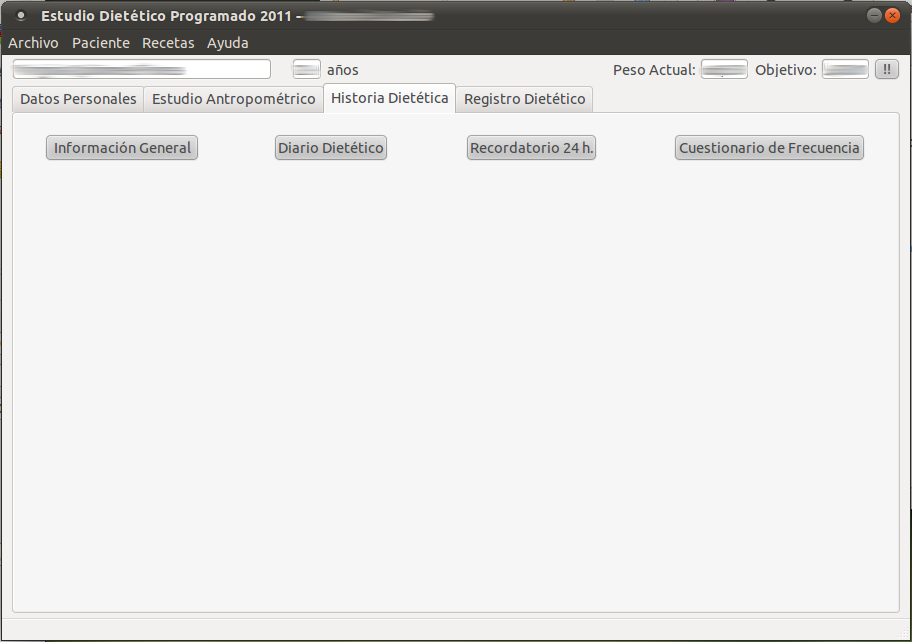
\includegraphics[scale=0.5]{../../Image/paciente-hist.png}
  \end{center}
  \caption{Capa de presentación: Pestaña Historia Dietética}
\end{figure}
\newpage
\item \textbf{Registro Dietético}: desde aquí se realizarán los semanarios que sirven de guía al paciente y le enseña a tener una buena alimentación, el cual es el mayor propósito de la aplicación.\\\\
\begin{figure}[H]
  \label{registro}
  \begin{center}
    % Comentar si no está el paquete tkiz instalado, y descomentar la
    % linea siguiente. Comentar además la inclusión del paquete en
    % estilos/estiloBase.sty
    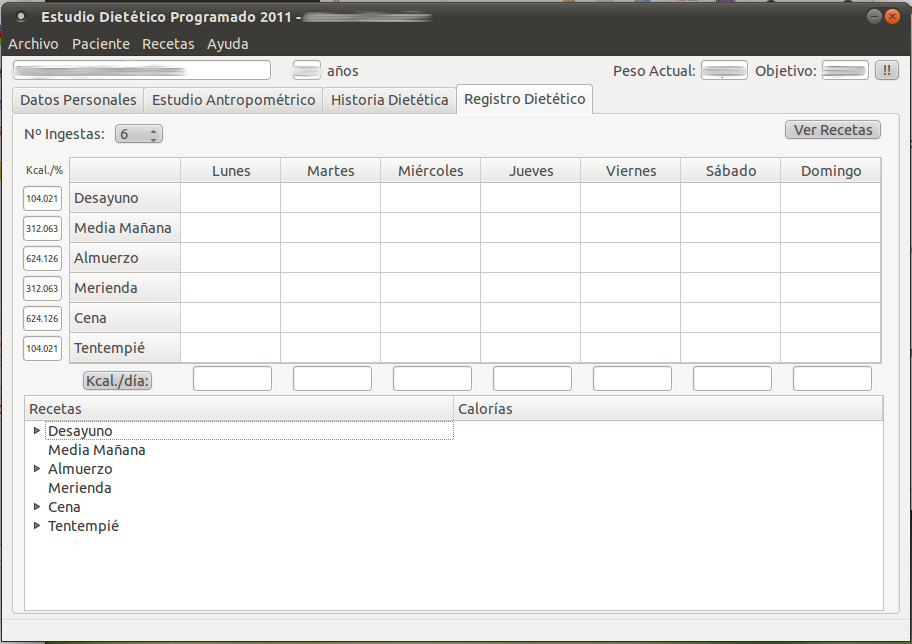
\includegraphics[scale=0.5]{../../Image/paciente-registro.png}
  \end{center}
  \caption{Capa de presentación: Pestaña Registro Dietético}
\end{figure}
\end{itemize}
\newpage
\item \textbf{Formularios de registro}: formulario para introducir datos en el sistema, en este caso, para el alta de un paciente. Se compone de los siguientes elementos:
\begin{itemize}
\item \textbf{Etiquetas identificativas}: indican el dato a introducir.
\item \textbf{Campo de texto}: donde el dietista introduce los datos.
\item \textbf{Botones de opción}: albergando los botones aceptar, que guardará los datos y el botón cancelar, que cancela el proceso.
\end{itemize}
\begin{figure}[H]
  \label{pnuevo}
  \begin{center}
    % Comentar si no está el paquete tkiz instalado, y descomentar la
    % linea siguiente. Comentar además la inclusión del paquete en
    % estilos/estiloBase.sty
    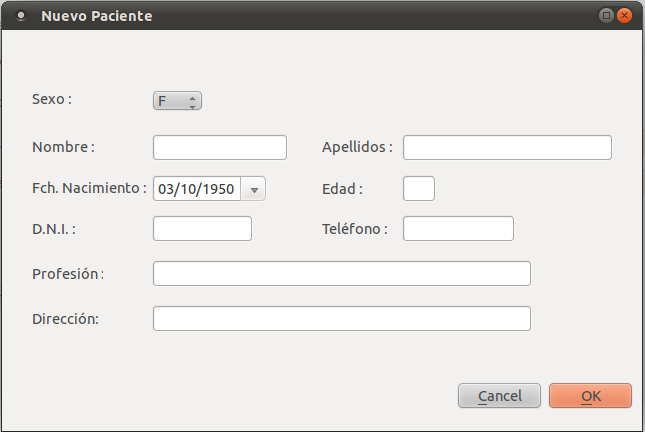
\includegraphics[scale=0.5]{../../Image/paciente-nuevo1.png}
  \end{center}
  \caption{Capa de presentación: Formulario Nuevo Paciente}
\end{figure}

\item \textbf{Nueva Receta}: formulario asociado al alta de una nueva receta. Éste cuenta con campos distintos al anterior, que se detallan a continuación:
\begin{itemize}
\item \textbf{Etiquetas identificativas}: indican el dato a introducir.
\item \textbf{Campos de texto}: donde el dietista introduce los datos.
\item \textbf{Selección de ingredientes}: selección de los ingredientes que forman parte de la receta.
\item \textbf{Desplegable de selección}: desplegable de categoría de receta.
\end{itemize}
\begin{figure}[H]
  \label{nreceta}
  \begin{center}
    % Comentar si no está el paquete tkiz instalado, y descomentar la
    % linea siguiente. Comentar además la inclusión del paquete en
    % estilos/estiloBase.sty
    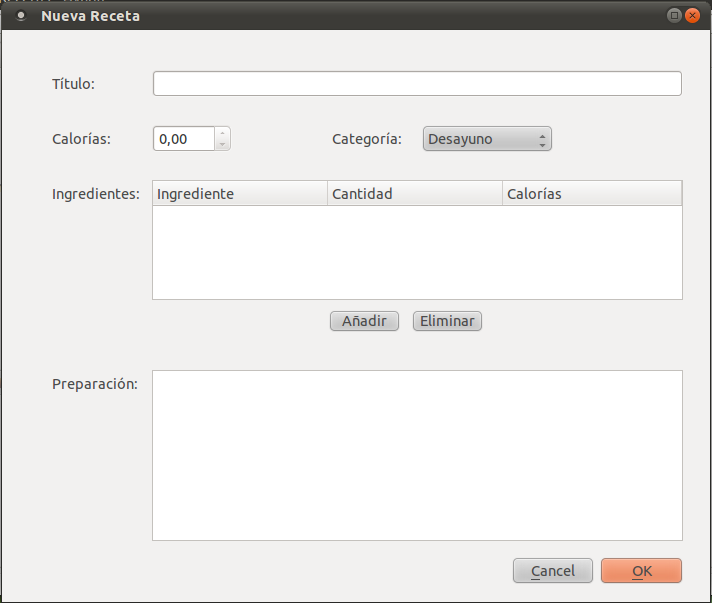
\includegraphics[scale=0.5]{../../Image/receta-nueva.png}
  \end{center}
  \caption{Capa de presentación: Formulario Nueva Receta}
\end{figure}
\end{itemize}

\section{Diseño de la base de datos}
\subsection{Diseño conceptual de la base de datos}
\begin{itemize}
\item Tipos de entidades:\\\\
A continuación se exponen las distintas entidades que intervendrán en la aplicación, así como los atributos que poseen cada una de ellas. \\
\begin{table}[H]
\begin{center}
  \begin{tabular}{| l | p{12cm} |}
    \hline
    Entidad & Atributos \\ \hline
    Dietista & Dni, Nombre, Password \\ \hline
    Paciente & Id\_paciente, Sexo, Dni, Nombre, Apellidos, Fch\_Nac, Tlf, Profesion, Direccion \\ \hline
	Antrop\_Nec & Id\_antropnec, Peso, Altura, Imc, Objetivo, Cadera, Cintura, Plieguetric, Complexion, Pesopactado, Mb, Actividad, EnergiaTotal, NumIngesta, PerdidaMatGrasa, InformacionTrat \\ \hline
	Analisis & Id\_analisis, Ruta, Nombre, Fecha \\ \hline
	Diario\_Dietetico & Id\_diario, Ruta, Nombre, Fecha \\ \hline
	Recordatorio & Id\_recordatorio, Ruta, Nombre, Fecha \\ \hline
	Info\_Gen & Id\_ig, camporegistro, contenidoregistro \\ \hline
	Trat\_Apoyo & Id\_tratapoyo, Fecha, Tratamiento, Psologia, Observaciones \\ \hline
	Peso\_Ideal & Id\_pesoideal, Fm, Complexion, Altura, Peso \\ \hline
	Receta & Id\_receta, Nombre, Calorias, Categoria, Preparacion \\ \hline
	Ingrediente & Id\_ingrediente, Nombre, Cantidad, Tipo, Calorias \\ \hline
	Enfermedad & Id\_enfermedad, Nombre \\ \hline
	Semanario & Id\_semanario, Lunes, Martes, Miercoles, Jueves, Viernes, Sabado, Domingo, kcal\_dia, Fecha, Kcalorias, Numingestas \\
	\hline
  \end{tabular}
\end{center}
\caption{Tabla de entidades}
\end{table}
\item Tipo de relaciones:\\\\
Las relaciones intervinientes son:
\begin{itemize}
\item \textbf{Pertenece a}: Relación que existe entre los dietistas y los pacientes.
\item \textbf{Posee}: Relación que existe entre los pacientes y los semanarios.
\item \textbf{Pacede}: Relación que existe entre los pacientes y las enfermedades.
\item \textbf{Tiene}: Relación que existe entre los semanarios y las recetas.
\item \textbf{Es autor de}: Relación que existe entre los dietistas y las recetas.
\item \textbf{Prohibe}: Relación que existe entre las enfermedades y los ingredientes.
\item \textbf{Necesita}: Relación que existe entre los ingredientes y las recetas.
\item \textbf{Es su}: Relación que existe entre los pesos ideales y los pacientes.
\item \textbf{Le corresponde}: Relación que existe entre las necesidades antropométricas y los pacientes.
\item \textbf{Realiza}: Relación que existe entre los diarios dietéticos y los pacientes.
\item \textbf{Recuerda}: Relación que existe entre los recordatorios y los pacientes.
\item \textbf{Se hace}: Relación que existe entre los análisis y los pacientes.
\item \textbf{Prefiere}: Relación que existe entre los ingredientes y los pacientes.
\item \textbf{Informa}: Relación que existe entre las informaciones generales y los pacientes.
\item \textbf{Toma}: Relación que existe entre los tratamientos de apoyo y los pacientes.
\end{itemize}

\newpage
\item Diagrama Entidad-Relación:\\
Para mayor comprensión del diagrama se omiten los atributos proporcionados en la tabla de entidades.
\begin{figure}[H]
  \label{d_er}
  \begin{center}
    % Comentar si no está el paquete tkiz instalado, y descomentar la
    % linea siguiente. Comentar además la inclusión del paquete en
    % estilos/estiloBase.sty
    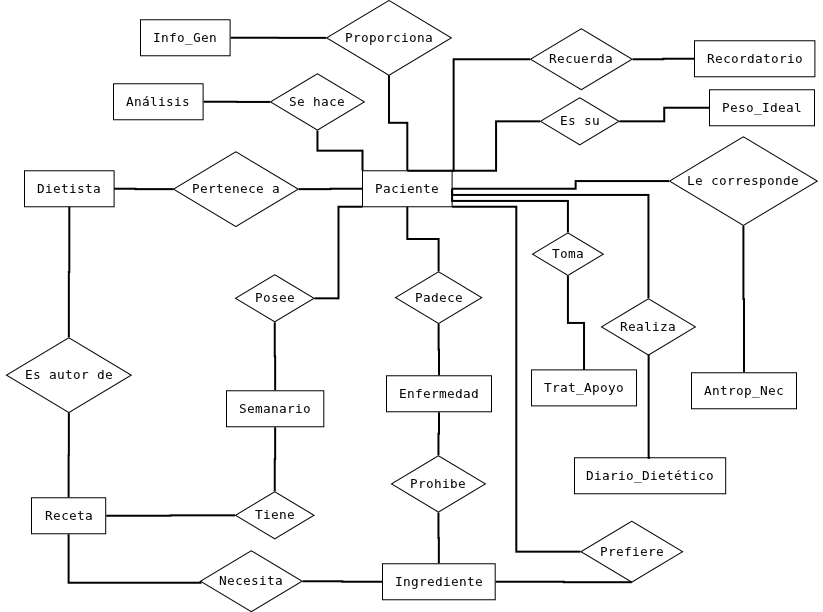
\includegraphics[scale=0.6]{../img/Diagrama_ER.png}
  \end{center}
  \caption{Diagrama Entidad Relación}
\end{figure}
\end{itemize}
\newpage
\subsection{Diseño lógico de la base de datos}
Después de realizar el estudio lógico de la base de datos, las tablas resultantes son:
\begin{itemize}
\item \textbf{Dietista}: (Dni, Nombre, Password)
\begin{itemize}
\item Clave primaria: \textit{Dni}
\item Se incluye \textit{Dni} en las tablas ``Paciente'', ``Receta'' y ``Receta\_Ingredientes''
\end{itemize}
\item \textbf{Paciente}: (Id\_paciente, Sexo, Dni, Nombre, Apellidos, Fch\_Nac, Tlf, Profesion, Direccion, Dni\_Diet)
\begin{itemize}
\item Clave primaria: \textit{Id\_paciente}
\item Clave foránea: \textit{Dni\_Diet}
\item Se incluye \textit{Id\_paciente} en las tablas ``Análisis'', ``Antrop\_Nec'', ``Diario\_Diet'', ``Enf\_Paciente'', ``Info\_gen'', ``Recordatorio'', ``Preferencia'', ``Semanario'' y ``Trat\_Apoyo''
\end{itemize}
\item \textbf{Antrop\_Nec}: (Id\_antropnec, Peso, Altura, Imc, Objetivo, Cadera, Cintura, Plieguetric, Complexion, Pesopactado, Mb, Actividad, EnegiaTotal, NumIngesta, PerdidaMatGrasa, InformacionTrat, Id\_paciente)
\begin{itemize}
\item Clave primaria: \textit{Id\_antropnec}
\item Clave foránea: \textit{Id\_paciente}
\end{itemize}
\item \textbf{Analisis}: (Id\_analisis, Ruta, Nombre, Fecha, Id\_paciente)
\begin{itemize}
\item Clave primaria: \textit{Id\_analisis}
\item Clave foránea: \textit{Id\_paciente}
\end{itemize}
\item \textbf{Diario\_Dietetico}: (Id\_diario, Ruta, Nombre, Fecha, Id\_paciente)
\begin{itemize}
\item Clave primaria: \textit{Id\_diario}
\item Clave foránea: \textit{Id\_paciente}
\end{itemize}
\item \textbf{Recordatorio}: (Id\_recordatorio, Ruta, Nombre, Fecha, Id\_paciente)
\begin{itemize}
\item Clave primaria: \textit{Id\_recordatorio}
\item Clave foránea: \textit{Id\_paciente}
\end{itemize}
\item \textbf{Info\_Gen}: (Id\_ig, camporegistro, contenidoregistro, Id\_paciente)
\begin{itemize}
\item Clave primaria: \textit{Id\_ig}
\item Clave foránea: \textit{Id\_paciente}
\end{itemize}
\item \textbf{Trat\_Apoyo}: (Id\_tratapoyo, Fecha, Tratamiento, Psologia, Observaciones, Id\_paciente)
\begin{itemize}
\item Clave primaria: \textit{Id\_tratapoyo}
\item Clave foránea: \textit{Id\_paciente}
\end{itemize}
\item \textbf{Peso\_Ideal}: (Id\_pesoideal, Fm, Complexion, Altura, Peso, Id\_paciente)
\begin{itemize}
\item Clave primaria: \textit{Id\_pesoideal}
\item Clave foránea: \textit{Id\_paciente}
\end{itemize}
\item \textbf{Receta}: (Id\_receta, Nombre, Calorias, Categoria, Preparacion, Dni\_Diet)
\begin{itemize}
\item Clave primaria: \textit{Id\_receta}
\item Clave foránea: \textit{Dni\_Diet}
\item Se incluye \textit{Nombre} en la tabla ``Receta\_Ingredientes''
\end{itemize}
\item \textbf{Ingrediente}: (Id\_ingrediente, Nombre, Cantidad, Tipo, Calorias)
\begin{itemize}
\item Clave primaria: \textit{Id\_ingrediente}
\item Se incluye \textit{Id\_Ingrediente} en la tabla ``Enf\_Ingred'', se incluye \textit{Nombre} en la tabla ``Receta\_Ingredientes''
\end{itemize}
\item \textbf{Receta\_Ingredientes}: (Id\_recing, NombreRec, NombreIngred, CantIngred, CalIngred, Dni\_Diet)
\begin{itemize}
\item Clave primaria: \textit{Id\_recing}
\item Clave foránea: \textit{Dni\_Diet}, \textit{NombreRec}, \textit{NombreIngred}
\end{itemize}
\item \textbf{Enfermedad}: (Id\_enfermedad, Nombre)
\begin{itemize}
\item Clave primaria: \textit{Id\_enfermedad}
\item Se incluye \textit{Id\_enfermedad} en las tablas ``Enf\_Ingred'' y ``Enf\_Paciente''
\end{itemize}
\item \textbf{Enf\_Ingred}: (Id\_enfingred, Id\_enfermedad, Id\_ingrediente)
\begin{itemize}
\item Clave primaria: \textit{Id\_enfingred}
\item Clave foránea: \textit{Id\_enfermedad} e \textit{Id\_ingrediente}
\end{itemize}
\item \textbf{Enf\_Paciente}: (Id\_enfpac, Id\_paciente, Id\_enfermedad)
\begin{itemize}
\item Clave primaria: \textit{Id\_enfpac}
\item Clave foránea: \textit{Id\_enfermedad} e \textit{Id\_paciente}
\end{itemize}
\item \textbf{Semanario}: (Id\_semanario, Lunes, Martes, Miercoles, Jueves, Viernes, Sabado, Domingo, kcal\_dia, Fecha, Kcalorias, Numingestas, Id\_paciente)
\begin{itemize}
\item Clave primaria: \textit{Id\_semanario}
\item Clave foránea: \textit{Id\_paciente}
\end{itemize}
\end{itemize}
Una vez obtenidas las tablas, se va a proceder a la normalización.\\
La normalización de la base de datos es una serie de reglas que permiten a los diseñadores de bases de datos desarrollar un esquema que minimice los problemas de lógica.\\
Una base de datos normalizada ofrece mayor comprensión de la misma y ocupa un espacio menor debido a la menor repetición de datos.\\\\
En nuestra base de datos se van a aplicar 3 grados de normalización, los cuales son:
\begin{itemize}
\item \textbf{1ª Forma Normal}: establece que todos los atributos de la tabla deben ser atómicos (indivisibles),
existe una clave primaria con atributos y estos son no nulos. Con esto se consiguen eliminar los valores repetidos en una base de datos.
\item \textbf{2ª Forma Normal}: establece que aquellos datos que no dependen de la clave primaria se deben eliminar y separar dentro de sus propias tablas.
\item \textbf{3ª Forma Normal}: una tabla esta en 3ª Forma Normal si todos los datos son dependientes funcionalmente de la clave primaria y no existe dependencias transitivas, es decir, que una columna dependa de otra y ninguna de ellas sea clave primaria.
\end{itemize}

A continuación se aplicarán los 3 grados de normalización a las tablas obtenidas previamente:

\begin{itemize}
\item \textbf{1ª Forma Normal}: todas las tablas se encuentran en 1ª Forma Normal, porque todos sus atributos son atómicos, y tienen una única clave primaria no nula.
\item \textbf{2ª Forma Normal}: todas las tablas se encuentran en 2ª Forma Normal, puesto que estan en 1ª Forma Normal y su clave primaria es un único atributo.
\item \textbf{3ª Forma Normal}: en este caso, en la tabla ``Antrop\_Nec'' observamos que el campo ``Imc'' depende de los campos ``Peso'' y ``Altura'', así mismo el campo ``Mb'' depende de los campos ``Objetivo'' y ``Complexion'', y también se observa que el campo ``EnergiaTotal'' depende de los campos ``Mb'' y ``Actividad''.
Para solucionar el problema podríamos dividir la tabla de modo que cumpliera la 3ª Forma Normal, tal que así:

\begin{table}[H]
\begin{center}
  \begin{tabular}{| l | p{8cm} |}
    \hline
    Entidad & Atributos \\ \hline
	Antrop\_Nec & Id\_antropnec, Peso, Altura, Objetivo, Cadera, Cintura, Plieguetric, Complexion, Pesopactado, Actividad, NumIngesta, PerdidaMatGrasa, InformacionTrat \\ \hline
	Imc\_Paciente & Id\_imc, Imc, Id\_antropnec \\ \hline
	Mb\_Paciente & Id\_mb, Mb, Id\_antropnec \\ \hline
	ET\_Paciente & Id\_et, EnergiaTotal, Id\_antropnec \\
	\hline
  \end{tabular}
\end{center}
\caption{Normalización 3º Forma Normal}
\end{table}
\end{itemize}

A continuación se muestran las tablas después del proceso de normalización. Para mayor comprensión las claves primarias aparecen subrayadas y las claves foráneas aparecen en cursiva.

\begin{table}[H]
\begin{center}
  \begin{tabular}{| l | p{12cm} |}
    \hline
    Entidad & Atributos \\ \hline
    Dietista & \underline{Dni}, Nombre, Password \\ \hline
    Paciente & \underline{Id\_paciente},  Sexo, Dni, Nombre, Apellidos, Fch\_Nac, Tlf, Profesion, Direccion, \textit{Dni\_Diet} \\ \hline
	Antrop\_Nec & \underline{Id\_antropnec}, Peso, Altura, Objetivo, Cadera, Cintura, Plieguetric, Complexion, Pesopactado, Actividad, NumIngesta, PerdidaMatGrasa, InformacionTrat, \textit{Id\_paciente} \\ \hline
	Imc\_Paciente & \underline{Id\_imc}, Imc, \textit{Id\_antropnec} \\ \hline
	Mb\_Paciente & \underline{Id\_mb}, Mb, \textit{Id\_antropnec} \\ \hline
	ET\_Paciente & \underline{Id\_et}, EnergiaTotal, \textit{Id\_antropnec} \\ \hline
	Analisis & \underline{Id\_analisis}, Ruta, Nombre, Fecha, \textit{Id\_paciente} \\ \hline
	Diario\_Dietetico & \underline{Id\_diario}, Ruta, Nombre, Fecha, \textit{Id\_paciente} \\ \hline
	Recordatorio & \underline{Id\_recordatorio}, Ruta, Nombre, Fecha, \textit{Id\_paciente} \\ \hline
	Info\_Gen & \underline{Id\_ig}, camporegistro, contenidoregistro, \textit{Id\_paciente} \\ \hline
	Trat\_Apoyo & \underline{Id\_tratapoyo}, Fecha, Tratamiento, Psologia, Observaciones, \textit{Id\_paciente} \\ \hline
	Peso\_Ideal & \underline{Id\_pesoideal}, Fm, Complexion, Altura, Peso, \textit{Id\_paciente} \\ \hline
	Receta & \underline{Id\_receta}, Nombre, Calorias, Categoria, Preparacion, \textit{Dni\_Diet} \\ \hline
	Ingrediente & \underline{Id\_ingrediente}, Nombre, Cantidad, Tipo, Calorias \\ \hline
	Receta\_Ingredientes & \underline{Id\_recing}, NombreRec, NombreIngred, CantIngred, CalIngred, \textit{Dni\_Diet} \\ \hline
	Enfermedad & \underline{Id\_enfermedad}, Nombre \\ \hline
	Enf\_Ingred & \underline{Id\_enfingred}, \textit{Id\_enfermedad}, \textit{Id\_ingrediente} \\ \hline
	Enf\_Paciente & \underline{Id\_enfpac}, \textit{Id\_paciente}, \textit{Id\_enfermedad} \\ \hline
	Semanario & \underline{Id\_semanario}, Lunes, Martes, Miercoles, Jueves, Viernes, Sabado, Domingo, kcal\_dia, Fecha, Kcalorias, Numingestas, \textit{Id\_paciente} \\
	\hline
  \end{tabular}
\end{center}
\caption{Tablas normalizadas}
\end{table}

\subsection{Diseño físico de la base de datos}
Una vez tenemos las tablas normalizadas con las que trabajaremos pasamos a la implementación de las mismas.
Observamos que durante la normalización creamos tablas nuevas, llamadas ``Imc\_Paciente'', ``Mb\_Paciente'' y ``ET\_Paciente'', pero realmente no optimizan el diseño ni la comprensión de las tablas.\\
Por tanto desnormalizaremos dichas tablas volviendo a incluir los respectivos campos en las tablas de las que provenían, ``Antrop\_Nec'', eliminando así las tablas ``Imc\_Paciente'', ``Mb\_Paciente'' y ``ET\_Paciente''.

\begin{table}[H]
\begin{center}
  \begin{tabular}{| l | p{12cm} |}
    \hline
    Entidad & Atributos \\ \hline
    Antrop\_Nec & \underline{Id\_antropnec}, Peso, Altura, Imc, Objetivo, Cadera, Cintura, Plieguetric, Complexion, Pesopactado, Mb, Actividad, EnergiaTotal, NumIngesta, PerdidaMatGrasa, InformacionTrat, \textit{Id\_paciente} \\ 
	\hline
  \end{tabular}
\end{center}
\caption{Tabla ``Antrop\_Nec'' desnormalizada}
\end{table}

\newpage

%
%\section{Diseño de la arquitectura}
%En esta sección se define la arquitectura general del sistema de información, especificando las distintas particiones físicas del mismo, la descomposición lógica en subsistemas de diseño y la ubicación de cada subsistema en cada partición, así como la especificación detallada de la infraestructura tecnológica necesaria para dar soporte al sistema de información.
%
%\subsection{Arquitectura física}
%En este apartado, describimos los principales componentes hardware que forman la arquitectura física de nuestro sistema, recogiendo por un lado los componentes de servidor y los componentes de sistemas externos con los que colabora nuestro sistema y por otro, los componentes hardware de cliente.
%
%\subsection{Arquitectura lógica}
%La arquitectura lógica del sistema está formada por los elementos software (servicios, aplicaciones, librerías, frameworks, etc.) que componen el software base, más el software desarrollado para cumplir los requisitos de la aplicación. También, se recogen los componentes de sistemas externos con los que interactúa nuestro sistema, así como los componentes software del lado cliente.
%
%\subsection{Arquitectura de diseño}
%La arquitectura de diseño especifica la forma en que los artefactos software de más bajo nivel, interactúan entre sí para lograr el comportamiento deseado en el sistema. Utilizaremos el patrón arquitectónico  Layers (Capas), con el cual estructuramos el sistema en un número apropiado de capas, de forma que todos los componentes de una misma capa trabajan en el mismo nivel de abstracción y los servicios proporcionados por la capa superior utilizan internamente los servicios proporcionados por la capa inmediatamente inferior.
%
%\subsubsection{Capa de presentación}
%Este grupo de artefactos software conforman la capa de presentación del sistema, incluyendo tanto los componentes de la vista como los elementos de control de la misma.
%\subsubsection{Capa de negocio}
%Este grupo de artefactos software conforman la capa de negocio del sistema, incluyendo los elementos del modelo de dominio y los servicios (operaciones del sistema).
%\subsubsection{Capa de integración}
%Este grupo de artefactos software conforman la capa de integración del sistema, incluyendo las clases de abstracción para el acceso a datos (BD o sistema de ficheros) o a sistemas heredados.
%\subsubsection{Servicios transversales}
%Este grupo de artefactos software pueden ser usados por elementos de cualquiera de las capas del sistema y fundamentalmente proporcionan servicios relacionados con requisitos no funcionales (calidad).
%
%
%\section{Diseño de la interfaz de usuario} 
%En esta sección se especifican las interfaces entre el sistema y el usuario, detallando el aspecto y el comportamiento de las diferentes pantallas e informes, de acuerdo con el entorno tecnológico definido. Con respecto a las pantallas e informes, es preciso realizar un prototipo o mockup gráfico. Junto a estos bocetos hay que definir qué ocurre en los distintos componentes visuales de la interfaz cuando aparecen y qué acciones se disparan cuando el usuario trabaja con ellas.
%Además, es preciso elaborar un diagrama de navegación, reflejando la secuencia de pantallas a las que tienen acceso los diferentes roles de usuario y la conexión entre éstas. 
%
%
%\section{Diseño de datos}
%En esta sección se define la estructura física de datos que utilizará el sistema, a partir del modelo de conceptual de clases, de manera que teniendo presente los requisitos establecidos para el sistema de información y las particularidades del entorno tecnológico, se consiga un acceso eficiente de los datos. La estructura física se compone de tablas, índices, procedimientos almacenados, secuencias y otros elementos dependientes del SGBD a utilizar.
%
%
%\section{Diseño de componentes}
%En esta sección se definen los componentes software necesarios para la implementación del sistema. Para facilitar la comprensión y la posterior implementación del sistema, es recomendable organizarlo en forma de subsistemas, los cuales se compondrán a su vez de módulos. Estos módulos (o paquetes) contendrán un conjunto de artefactos software, que representaremos en forma de clases y que corresponderán a una de las capas identificadas en la arquitectura. 
%Para cada uno de los módulos funcionales del sistema debemos realizar un diagrama de secuencia, para definir la interacción existente entre las clases de objetos que permitan responder a eventos externos. A partir de este diagrama, se genera el diagrama de clases de diseño, incluyendo los elementos del modelo conceptual, enriquecidos con las nuevas clases, relaciones, atributos y operaciones resultantes. Asimismo, se detallará el comportamiento de las operaciones más relevantes.
%
%
%\section{Parametrización del software base}
%En esta sección, se detallan las modificaciones a realizar sobre el software base, que son requeridas para la correcta construcción del sistema. En esta sección incluiremos las  actuaciones necesarias sobre la interfaz de administración del sistema, sobre el código fuente o sobre el modelo de datos.
%
%
%
%
%
%
%
%
%
%
%
%
%
%


\chapter{Implementación del Sistema}
% ------------------------------------------------------------------------------
% Este fichero es parte de la plantilla LaTeX para la realización de Proyectos
% Final de Grado, protegido bajo los términos de la licencia GFDL.
% Para más información, la licencia completa viene incluida en el
% fichero fdl-1.3.tex

% Copyright (C) 2012 SPI-FM. Universidad de Cádiz
% ------------------------------------------------------------------------------

A continuación se detallan algunos aspectos referentes al desarrollo de la aplicación:

\section{Entorno tecnológico}
Para el desarrollo se ha utilizado las siguientes herramientas:
\begin{itemize}
\item \textit{Emacs}: Editor de texto muy potente, usado para generar los archivos \textit{Python}(``.py''). Este IDE abarca cualidades como resaltado de sintaxis, soporte multidocumento, consola integrada, ...
\item \textit{Python}: Lenguaje de programación utilizado para el desarrollo, en su versión 2.7.1. Junto a \textit{Python} se han utilizado las siguientes bibliotecas:
\begin{itemize}
\item \textit{PyQt}: adaptación de la biblioteca gráfica \textit{Qt}, necesario para la interfaz de usuario.
\item \textit{Relatorio}: Permite generar informes a través de plantillas ``.odt''. \textit{Relatorio} necesita de la biblioteca \textit{OpenOffice-Python} para interactuar con \textit{OpenOffice}.
\item \textit{Poppler}: en la versión de la biblioteca \textit{popplerqt4}. Utilizada para generar archivos PDFs desde nuestra aplicación.
\end{itemize}
\item \textit{Qt4 Designer}: diseñador de interfaces gráficas para \textit{Qt}. Con esta herramienta generamos los archivos ``.ui'', que representan las pantalla y formularios de la aplicación. Posteriormente se usa el comando \textit{pyuic4} que transformará los archivos ``.ui'' en archivos ``.py''.
\item \textit{Git}: usado para el control de versiones. En este caso haciendo uso de las ventajas de \textit{Git}, obteniendo el control de versiones en local y otro en servidor con las versiones acabadas.
\end{itemize}

\section{Código fuente}
Para la implementación del código fuente se ha optado por la siguiente distribución de directorios:
\begin{itemize}
\item \textbf{usr/share/edp11}: directorio principal donde se encuentran los archivos principales ``.py'' de la aplicación. Cada archivo representa una clase implicada en la aplicación.
\item \textbf{edp11/PY\_UIs}: directorio en el que se encuentran todas las transformaciones de los archivos ``.ui'' en ``.py'' de la interfaz gráfica, necesarios para la ejecución de la aplicación. Cada uno de ellos representa una pantalla o formulario de la aplicación.
\item \textbf{edp11/Docu}: directorio en el que se encuentran las plantillas ``.odt'' necesarias para la generación de los archivos PDFs de la aplicación, así como PDFs pertenecientes a la aplicación siendo estos documentos del dietista que debe proporcionar.
\end{itemize}


\section{Problemas ocurridos durante la implementación}
A la hora de implementar la aplicación surgieron diversos problemas, causados principalmente por el desconocimiento de las herramientas usadas, así como del lenguaje de programación \textit{Python} (absolutamente algo nuevo para mí). En el caso de \textit{Python}, existe numerosa cantidad de documentación, tanto en su web oficial como en foros y blogs, por lo que acostumbrarse fue cuestión rápida.\\\\
En el caso de \textit{PyQt}, el aprendizaje resultó más difícil, debido a su escasa documentación. Hubo que recurrir a la documentación de \textit{Qt} así como a foros para solvertar dudas y problemas. \\
Hubo que declarar nuevos tipos de elementos para un comportamiento de los objetos acorde con lo requerido.\\\\
Otro caso es la biblioteca \textit{Relatorio}, que para operar con ella había que determinar como formatear los datos de entrada, lo cual fue laborioso.\\\\
Sin hablar de la biblioteca \textit{Poppler}, para la que la utilización en \textit{Python} debía seguir una forma, y no fue encontrada en ninguna documentación ni foro ni blog, finalmente tomando como referencia la poca documentación oficial, y haciendo un estudio lógico de la utilización se llegó con éxito.













\chapter{Pruebas del Sistema}
% ------------------------------------------------------------------------------
% Este fichero es parte de la plantilla LaTeX para la realización de Proyectos
% Final de Grado, protegido bajo los términos de la licencia GFDL.
% Para más información, la licencia completa viene incluida en el
% fichero fdl-1.3.tex

% Copyright (C) 2012 SPI-FM. Universidad de Cádiz
% ------------------------------------------------------------------------------

Para comprobar el correcto funcionamiento de la aplicación, tanto de la gestión de datos como la ejecución correcta, se ha realizado una serie de pruebas.\\
Las pruebas realizadas se han llevado a cabo manualmente. A continuación se explicarán más en detalle la forma de realizar las distintas pruebas.\\

\section{Pruebas de caja negra}

Para las pruebas de caja negra, realizamos las pruebas independientes y las pruebas sobre subsistemas.

\subsection{Independientes}
Se llevaron a cabo pruebas de caja negra sobre aquellos objetos que interactúan directamente sobre la base de datos y son independientes de otros objetos. En este tipo de pruebas no se tienen en cuenta la implementación, sino los datos de entrada y la salida que se produce.\\\\
Se observaron los valores recogidos del módulo que estabamos probando, antes de su interactuación con la base de datos, para ello, mediante la consola e impresiones de los valores recogidos se verificaba el correcto funcionamiento, posteriormente se corroboraba que los datos habían actuado de forma correcta en la base de datos, a través del \textit{SQLite Manager}, plugin para \textit{Firefox}, que facilita la consulta de la base de datos de manera más visual.

\subsection{Sobre subsistemas}
Al igual que con los objetos o módulos independientes, se realizaron pruebas de caja negra sobre aquellos subsistemas para comprobar el correcto funcionamiento. Este tipo de prueba nos permite comprobar si hay buena comunicación entre los elementos que forman el subsistema.\\\\
Primeramente se observaba que los botones e interactuaciones del módulo en cuestión funcionaban correctamente, comprobando que los campos se comportaban de forma correcta, así como se accedía a las ventanas de forma correcta a través de los botones correspondientes. Posteriormente mediante la consola nuevamente se imprimieron los valores de referencia, tales como las variables de sesión de dietista y paciente de las clases \textit{Dietista} y \textit{Paciente} respectivamente, que mantienen una jerarquía en la aplicación y un orden para la comprobación de acceso a datos del usuario.

\section{Pruebas de caja blanca}
Son pruebas dedicadas prácticamente en su totalidad a recorrer todas las posibles opciones o caminos que forman un proceso, con el fin de asegurarnos que todas las posibles opciones funcionan correctamente.\\
A cada incremento de la aplicación, se probaba nuevamente de forma manual que se mantenía el funcionamiento correcto, accediento a todas las ventanas y verificando todos los campos de los distintos módulos a los que se accedía, recorriendo en cada caso cada una de las posibles acciones que se podían realizar.\\\\
A medida que se implementaban nuevas funcionalidades en los distintos incrementos, en el caso de que interactuara con la base de datos se probaba primero en modo consola la órden para posteriormente integrarla en el código. El objetivo principal era comprobar el correcto tratamiento de la información, tanto en la obtención de datos como en almacenamiento de los mismos.\\
Cuando se finalizó la aplicación se probó nuevamente toda la interacción entre los módulos.

\section{Pruebas de sistema}
Se trata de ver la interacción correcta entre los distintos subsistemas que componen la aplicación.\\
Al igual que las pruebas de caja negra sobre subsistemas, se corroboró que todos los botones funcionaban a la perfección al igual que todos los campos se comportaban de forma correcta.\\\\ 
Las pruebas se realizaron sobre el sistema operativo \textit{Linux}, en sus distribuciones \textit{Ubuntu 10.10}, \textit{Ubuntu 11.04} y \textit{Ubuntu 12.04} sin ningún tipo de problema.\\
En este caso se realizó sobre la aplicación finalizada, comprobando el correcto funcionamiento e interactuación entre los subsistemas de la aplicación.\\\\
Se comenzó probando la gestión de dietistas y recetas, ya que son clases independientes. Esta gestión incluye altas, eliminaciones y modificaciones sobre los datos introducidos.\\
Posteriormente se comprobó la gestión de pacientes. Se comprobó, que la comunicación con la gestión de dietistas
era correcta.\\\\
Seguidamente se comprobó todos los casos referentes a la información del paciente; gestión de enfermedades, gestión de diarios dietéticos, recordatorios, información general, preferencias y semanarios. En esta parte se comprobó la creación de objetos y la comunicación e integración con la base de datos.\\
También se comprobaron nuevamente todos y cada uno de los elementos que componen la aplicación, botones, menús desplegables, pestañas, enlace entre ventanas, etc.

\section{Pruebas sobre la interfaz}

Para las pruebas sobre la interfaz, realizamos las pruebas de limitación en el tipo de campo, limitación en la longitud de los campos y limitación con respecto a campos vacíos.

\subsection{Limitación en el tipo de campo}
Se trata de limitar los caracteres introducidos por el usuario en un campo concreto. Por ejemplo, en el caso de teléfono introducir dígitos unicamente, el DNI sólo se permiten una serie de dígitos y una letra.\\\\
Se introdujeron manualmente todos los posibles casos que pudieran errar en la aplicación, contemplando que no hay ningún fallo en los tipos de campo.

\subsection{Limitación en la longitud de los campos}
Algunos campos tienen un número finito de dígitos o caracteres, por lo que también se comprueba que el usuario no introduce ni más ni menos valores de los esperados.\\\\
Debido a que la aplicación se realizó mediante el programa \textit{Qt4 Designer}, ya se especifica sobre éste la limitación sobre la longitud. Posteriormente fue probado manualmente para verificar el buen funcionamiento del diseño y de la aplicación.

\subsection{Limitación con respecto a campos vacíos}
Como algunos campos de la base de datos no aceptan valores nulos, en todos aquellos campos que sea necesario se comprueba que el valor no sea nulo.\\\\
Nuevamente se realizaron las pruebas manualmente, dejando a propósito campos vacíos para corroborar que se llevaba un buen control sobre ello, pudiendo observar el funcionamiento correcto, dando el aviso en todos los casos que son necesarios que no sean vacíos.

\section{Pruebas de aceptación}
Estas pruebas se han realizado por parte del cliente final, con la puesta en funcionamiento en fase de prueba de la aplicación, una vez comprobado su correcto funcionamiento mediante las pruebas anteriores.\\\\
Se realizaron en cada incremento, corroborando que el cliente final le satisfacía en cada uno de ellos. Finalmente, después de la última entrega, el cliente final ha empezado con la utilización de la aplicación, totalmente satisfecho con el funcionamiento, el diseño y el manejo de la aplicación.


% EPILOGO
\part{Epílogo}
\null\vfill

\chapter{Manual de usuario}
%fich.tex
%%%%%%%%%%%%%%%%%%%%%%%%%%%%%%%%%%%%%%%%%%%%%%%%%%%%%%%%%%%%%%%%%%%%%%%%
% Manuel González Pérez
% Descripción del documento:
	
%%%%%%%%%%%%%%%%%%%%%%%%%%%%%%%%%%%%%%%%%%%%%%%%%%%%%%%%%%%%%%%%%%%%%%%%


%%%%%%%%%%%%%%%%%%%%%%%%%%%%%%%%%%%%%%%%%%%%%%%%%%%%%%%%%%%%%%%%%%%%%%%%
%Clase de documento
\documentclass[12pt, spanish]{article}
%%%%%%%%%%%%%%%%%%%%%%%%%%%%%%%%%%%%%%%%%%%%%%%%%%%%%%%%%%%%%%%%%%%%%%%%


%%%%%%%%%%%%%%%%%%%%%%%%%%%%%%%%%%%%%%%%%%%%%%%%%%%%%%%%%%%%%%%%%%%%%%%%	
%Paquetes de lenguaje:
%%%%%%%%%%%%%%%%%%%%%%%%%%%%%%%%%%%%%%%%%%%%%%%%%%%%%%%%%%%%%%%%%%%%%%%%
\usepackage[utf8]{inputenc}
\usepackage[spanish]{babel}
\usepackage{graphicx}
%\usepackage[spanish, activeacute] {babel}	
%\usepackage[spanish]{babel} 				
%\usepackage[latin1]{inputenc}
%%%%%%%%%%%%%%%%%%%%%%%%%%%%%%%%%%%%%%%%%%%%%%%%%%%%%%%%%%%%%%%%%%%%%%%%


%%%%%%%%%%%%%%%%%%%%%%%%%%%%%%%%%%%%%%%%%%%%%%%%%%%%%%%%%%%%%%%%%%%%%%%%
%Paquetes para encabezados y pie de páginas
%%%%%%%%%%%%%%%%%%%%%%%%%%%%%%%%%%%%%%%%%%%%%%%%%%%%%%%%%%%%%%%%%%%%%%%%
\usepackage{fancyhdr}
%%%%%%%%%
% \pagestyle{fancy} %Si se cambia el estilo de página, antes de empezar 
	%el documento. Esto hace que el emcabezado y pie de página se 
	%quede separado del texto por una línea
%%%%%%%%%	
% \fancyhead{} % Límpia el texto que se está usando como encabezado
%%%%%%%%%
% \fancyhead[OPCIONES]{Encabezado}
	% OPCIONES:
		% L texto a la izquierda
		% C texto centrado
		% R texto a la derecha
		% E página par
		% O pagina impar
	%Ejemplo: 
		% fancyhead [LE] {"Doc. Latex"} 
			% Establece como emcabezado de las páginas pares "Doc Latex"
			% con alineacion a la izquierda
%%%%%%%%%			
% \fancyfoot[OPCIONES]{Píe de pag.}
	% OPCIONES:
		% L C R E O
	%Ejemplo
		% \fancyfoot[LE,RO]{\thepage} 
			% Establece como píe de pág. el número de página. con 
			% alineación a la izq en paginas pares y a la derecha en
			% las impares
%%%%%%%%%			
% \renewcommand{\headrulewidth}{0.4pt}
% \renewcommand{\footrulewidth}{0.4pt}
	% Fija el grosor de la la linea que separa el emcabezado y pie de pág
%%%%%%%%%
% Otros comandos:
%\lhead{}
%\chead{}
%\rhead{}
%\lfoot{}
%\cfoot{}
%%%%%%%%%%%%%%%%%%%%%%%%%%%%%%%%%%%%%%%%%%%%%%%%%%%%%%%%%%%%%%%%%%%%%%%%


%%%%%%%%%%%%%%%%%%%%%%%%%%%%%%%%%%%%%%%%%%%%%%%%%%%%%%%%%%%%%%%%%%%%%%%%
% Paquetes para tamaños y distancias
%%%%%%%%%%%%%%%%%%%%%%%%%%%%%%%%%%%%%%%%%%%%%%%%%%%%%%%%%%%%%%%%%%%%%%%%
\usepackage{anysize} 
%%%%%%%%%%%
% \marginsize{3cm}{2cm}{2cm}{2cm}
	% Controla los márgenes {izquierda}{derecha}{arriba}{abajo}. 
%%%%%%%%%%%%%%%%%%%%%%%%%%%%%%%%%%%%%%%%%%%%%%%%%%%%%%%%%%%%%%%%%%%%%%%%


%%%%%%%%%%%%%%%%%%%%%%%%%%%%%%%%%%%%%%%%%%%%%%%%%%%%%%%%%%%%%%%%%%%%%%%%
%Paquetes de carácteres especiales:
%%%%%%%%%%%%%%%%%%%%%%%%%%%%%%%%%%%%%%%%%%%%%%%%%%%%%%%%%%%%%%%%%%%%%%%%
%\usepackage{dsfont}	
%Para representar conjuntos matematicos comunes: Z, N, R...
	% mathds{R}, mathds{N},...
%%%%%%%%%%%%%%%%%%%%%%%%%%%%%%%%%%%%%%%%%%%%%%%%%%%%%%%%%%%%%%%%%%%%%%%%


%%%%%%%%%%%%%%%%%%%%%%%%%%%%%%%%%%%%%%%%%%%%%%%%%%%%%%%%%%%%%%%%%%%%%%%%
%Paquetes de color:
%%%%%%%%%%%%%%%%%%%%%%%%%%%%%%%%%%%%%%%%%%%%%%%%%%%%%%%%%%%%%%%%%%%%%%%%
\usepackage{color}
%%%%%%%%%%%%%%%%%%%%%%%%%%%%%%%%%%%%%%%%%%%%%%%%%%%%%%%%%%%%%%%%%%%%%%%%
%Definición de colores:
\definecolor{gray97}{gray}{.97}
\definecolor{gray75}{gray}{.75}
\definecolor{gray45}{gray}{.45}
%%%%%%%%%%%%%%%%%%%%%%%%%%%%%%%%%%%%%%%%%%%%%%%%%%%%%%%%%%%%%%%%%%%%%%%%


%%%%%%%%%%%%%%%%%%%%%%%%%%%%%%%%%%%%%%%%%%%%%%%%%%%%%%%%%%%%%%%%%%%%%%%%
%Paquete de listado de código:
%%%%%%%%%%%%%%%%%%%%%%%%%%%%%%%%%%%%%%%%%%%%%%%%%%%%%%%%%%%%%%%%%%%%%%%%
\usepackage{listings}
%%%%%%%%%%%%%%%%%%%%%%%%%%%%%%%%%%%%%%%%%%%%%%%%%%%%%%%%%%%%%%%%%%%%%%%%
%Configuración del listado:
\lstset { 
	frame=Ltb,
     framerule=0pt,
     aboveskip=0.1cm,
     framextopmargin=0.3pt,
     framexbottommargin=0.2pt,
     framexleftmargin=0.3cm,
     framesep=0pt,
     rulesep=.2pt,
     backgroundcolor=\color{gray97},
     rulesepcolor=\color{black},
     %
     stringstyle=\ttfamily,
     showstringspaces = false,
     basicstyle=\small\ttfamily,
     commentstyle=\color{gray45},
     keywordstyle=\bfseries,
   	%
     numbers=left,
     numbersep=1pt,
     numberstyle=\tiny,
     numberfirstline = false,
     breaklines=true,
}
%%%%%%%%%%%%%%%%%%%%%%%%%%%%%%%%%%%%%%%%%%%%%%%%%%%%%%%%%%%%%%%%%%%%%%%%


%%%%%%%%%%%%%%%%%%%%%%%%%%%%%%%%%%%%%%%%%%%%%%%%%%%%%%%%%%%%%%%%%%%%%%%%
%Estilo de página
%%%%%%%%%%%%%%%%%%%%%%%%%%%%%%%%%%%%%%%%%%%%%%%%%%%%%%%%%%%%%%%%%%%%%%%%
%\textwidth 6.75in								  %ancho de texto
%\oddsidemargin -0.2in							%margen izquierdo 
\parskip 0.2in									%espacio parrafos
%%%%%%%%%%%%%%%%%%%%%%%%%%%%%%%%%%%%%%%%%%%%%%%%%%%%%%%%%%%%%%%%%%%%%%%%


%%%%%%%%%%%%%%%%%%%%%%%%%%%%%%%%%%%%%%%%%%%%%%%%%%%%%%%%%%%%%%%%%%%%%%%%	
%datos del documento
%\title{Estudio Dietético Programado 2011\\Manual de Usuario}						%titulo
%\author{Manuel González Pérez}						%autor
%\date{}												%fecha
%%%%%%%%%%%%%%%%%%%%%%%%%%%%%%%%%%%%%%%%%%%%%%%%%%%%%%%%%%%%%%%%%%%%%%%%


%%%%%%%%%%%%%%%%%%%%%%%%%%%%%%%%%%%%%%%%%%%%%%%%%%%%%%%%%%%%%%%%%%%%%%%%
%Documento:
%%%%%%%%%%%%%%%%%%%%%%%%%%%%%%%%%%%%%%%%%%%%%%%%%%%%%%%%%%%%%%%%%%%%%%%%
\begin{document}
%%%%%%%%%%%%%%%%%%%%%%%%%%%%%%%%%%%%%%%%%%%%%%%%%%%%%%%%%%%%%%%%%%%%%%%%
%\maketitle
%\newpage
%\pagebreak 
\tableofcontents
\newpage
\section{Introducción}
Este manual pretende ser una guía para la correcta utilización del programa
de escritorio Estudio Dietético Programado 2011 (EDP11).
Este programa es un software para la realización de dietas personalizadas así
como el seguimiento del paciente en su evolución.
\newpage


\section{Presentación de la aplicación}
La aplicación esta orientada a dietistas profesionales con el fin de poder dar un buen servicio y seguimiento de sus pacientes.
Cuando el usuario inicia la aplicación se mostrará la pantalla principal de la misma. Desde ella se podrá acceder a las diferentes opciones ofrecidas, descritas a lo largo de este manual.
La aplicación contiene los siguientes componentes:
\begin{itemize}
\item \textbf{Barra de menú superior:} En dicha barra se mostrarán las distintas acciones posibles, habilitándose y deshabilitándose según la ejecución de la aplicación.
\item \textbf{Área de información rápida:} En dicha área se podrán observar el nombre, edad, peso actual y peso objetivo, así como un icono de información que determinará si hay información relevante para el tratamiento del paciente.
\item \textbf{Pestañas interiores de información e interactuación:} En dichas pestañas se obtendrán información del paciente a tratar así como aquello con lo que se pueda interactuar, separados en \textbf{Datos Personales}, \textbf{Estudio Antropométrico}, \textbf{Historia Dietética} y \textbf{Registro Dietético}
\end{itemize}
\includegraphics[scale=0.5]{Image/aplicacion.png} 
\newpage


\subsection{Barra de menú superior}

\includegraphics[scale=0.5]{Image/barra-superior.png}\\\\
La barra superior contiene los submenús:
\begin{itemize}
\item Archivo
\begin{itemize}
\item Abrir Perfil Dietista
\item Cerrar Perfil
\item Guardar
\item Imprimir
\item Salir
\end{itemize}
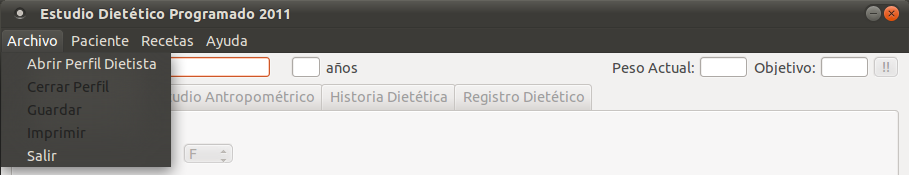
\includegraphics[scale=0.5]{Image/archivo-barra.png} 
\item Paciente
\begin{itemize}
\item Nuevo Paciente
\item Abrir Paciente
\item Cerrar Paciente
\item Eliminar Paciente
\end{itemize}
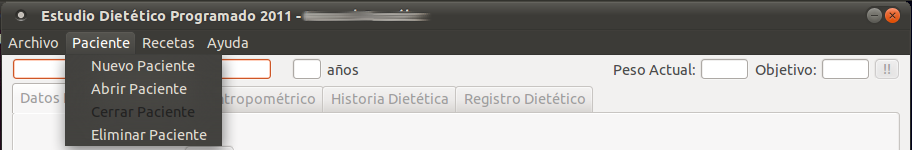
\includegraphics[scale=0.5]{Image/paciente-barra.png} 
\item Recetas
\begin{itemize}
\item Nueva Receta
\item Editar Receta
\item Eliminar Receta
\end{itemize}
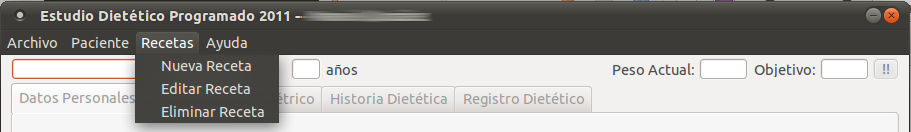
\includegraphics[scale=0.5]{Image/receta-barra.png} 
\item Ayuda
\begin{itemize}
\item Manual
\item Acerca de
\end{itemize}
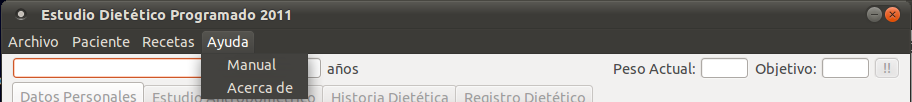
\includegraphics[scale=0.5]{Image/ayuda-barra.png} 
\end{itemize}



\subsubsection{Archivo}
\begin{enumerate}
\item \textbf{Abrir Perfil Dietista:}\\\\
Desde aquí se podrá seleccionar el perfil de dietista a abrir, así como crear un perfil nuevo o eliminar uno existente.\\\\
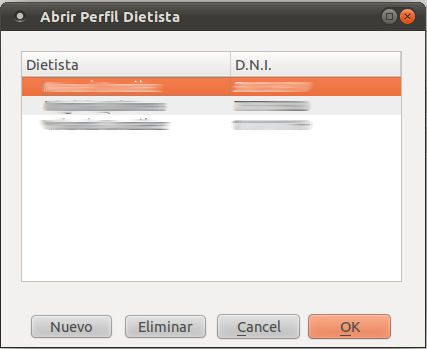
\includegraphics[scale=0.5]{Image/dietista-abrir.png}
\begin{enumerate}
\item \textit{Seleccionar perfil existente.}\\\\
Al seleccionar un perfil existente se pasará a la ventana de contraseña, en la cual habrá que introducir la contraseña correspondiente al perfil.\\\\
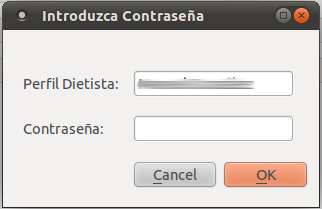
\includegraphics[scale=0.5]{Image/dietista-passwd.png}
\item \textit{Nuevo Perfil.}\\\\
Al seleccionar Nuevo se podrá incluir un nuevo perfil en el cual tendremos que rellenar los datos correspondientes así como elegir una contraseña para próximas insercciones.\\\\
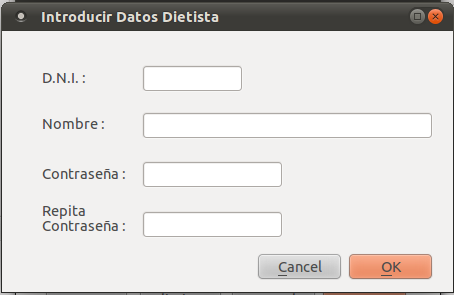
\includegraphics[scale=0.5]{Image/dietista-datos.png}
\item \textit{Eliminar Perfil.}\\\\
Si procede a eliminar un perfil existente accederá a la ventana de confirmación, en tal caso deberá introducir la clave de administración, la cual deberá solicitar al administrador (gonzalezperezmanuel@gmail.com)\\\\
\includegraphics[scale=0.5]{Image/dietista-eliminar.png}
\end{enumerate}
\item \textbf{Cerrar Perfil:}\\\\
Al seleccionar Cerrar Perfil se cerrará el perfil en ejecución actual.\\\\
\includegraphics[scale=0.5]{Image/dietista-cerrar.png}
\item \textbf{Guardar}\\\\
Al seleccionar Guardar se guardarán los cambios efectuados a lo largo del programa.
\item \textbf{Imprimir}\\\\
Al seleccionar Imprimir se imprimirá el semanario último guardado, así como las correspondientes elaboraciones de cada plato.\\\\
\includegraphics[scale=0.5]{Image/dietista-imprimir.png}
\item \textbf{Salir}\\\\
Al seleccionar Salir se saldrá de la aplicación.\\\\
\end{enumerate}
\newpage





\subsubsection{Paciente}
\begin{enumerate}
\item \textbf{Nuevo Paciente}\\\\
Al seleccionar Nuevo Paciente se podrá dar de alta a un paciente asociado al perfil de dietista actual.\\\\
\includegraphics[scale=0.5]{Image/paciente-nuevo1.png}\\\\
Una vez introducidos los datos, se pasará a la siguiente ventana.\\\\
\includegraphics[scale=0.5]{Image/paciente-nuevo2.png}\\\\
Desde esta ventana se podrá imprimir el \textit{Diario Dietético} y el \textit{Recordatorio 24 h.}; así como rellenar el \textit{Cuestionario de Frecuencia}.
\begin{enumerate}
\item \textit{Diario Dietético.}\\\\
El Diario Dietético se trata de un diario de 3 días el cual el paciente se deberá llevar a casa para rellenarlo siguiendo las instrucciones, apuntando todas las comidas que hace durante los días señalados.
\item \textit{Recordatorio 24 h.}\\\\
El Recordatorio 24 h. se trata de un diario de 1 día el cual el paciente deberá rellenar con lo que recuerde haber comido en el día anterior.
\item \textit{Cuestionario de Frecuencia.}\\\\
El Cuestionario de Frecuencia servirá para apuntar la frecuencia con la cual se consumen los alimentos, así como la preferencia puntuando de 1 a 5 sobre los mismos.\\\\
\includegraphics[scale=0.5]{Image/cuestfrec.png}\\\\
\end{enumerate}
\item \textbf{Abrir Paciente}\\\\
Al seleccionar Abrir Paciente se accederá a la ventana con el listado de los pacientes del dietista actual. Desde aquí se podrá seleccionar al paciente deseado.\\\\
\includegraphics[scale=0.5]{Image/paciente-abrir.png}\\\\
\item \textbf{Cerrar Paciente}\\\\
Desde aquí se cerrará el perfil de paciente actual.\\
\item \textbf{Eliminar Paciente}\\\\
Desde aquí se accederá al listado de pacientes, desde el cual se podrá eliminar el paciente seleccionado y así todos sus datos.\\\\
\includegraphics[scale=0.5]{Image/paciente-eliminar.png}\\\\
\end{enumerate}
\newpage





\subsubsection{Recetas}
\begin{enumerate}
\item \textbf{Nueva Receta}\\\\
Al seleccionar Nueva Receta se accederá a la ventana desde la cual elaborar una nueva receta perteneciente al perfil del dietista actual.\\\\
\includegraphics[scale=0.5]{Image/receta-nueva.png}\\\\
En la elaboración de la receta se rellenará el nombre, los ingredientes y las indicaciones para la preparación. 
\begin{enumerate}
\item \textit{Añadir Ingredientes}\\\\
Para añadir ingredientes se seleccionará Añadir, el cual accederá a la ventana de selección de ingredientes.\\\\
\includegraphics[scale=0.5]{Image/ingrediente-anadir.png}\\\\
Estos ingredientes estarán clasificados por grupos y alfabeticamente, ofreciendo una mejora en la búsqueda.
Desde aquí se podrá seleccionar el ingrediente y escribir la cantidad deseada para la receta.
En el caso de no encontrar un ingrediente u observar alguna errata en alguno de ellos, existen opciones para las operaciones respectivamente.\\\\
\begin{enumerate}
\item \textit{Nuevo}\\\\
Al seleccionar Nuevo, se accederá a la ventana desde la cual describir todo lo necesario para ingresar un nuevo ingrediente.\\\\
\includegraphics[scale=0.5]{Image/ingrediente-nuevo.png}\\\\
En dicha ventana se pedirá nombre del ingrediente, medida en la que se medirá, pudiendo ser 1, 10, 100 siendo unidad, mililitros y gramos respectivamente, tipo, donde se pondrá el grupo al que pertenece, y por último las calorías del ingrediente que comprenden la medida elegida.
\item \textit{Modificar}\\\\
Al seleccionar un ingrediente y posteriormente la opción Modificar, se podrá modificar cualquiera de los campos del ingrediente.\\\\
\includegraphics[scale=0.5]{Image/ingrediente-modificar.png}\\\\
Atención: Al modificar un ingrediente, quedarán modificadas todas las recetas en las que aparezca dicho ingrediente. Se recomienda revisarlas para evitar errores con respecto a las calorías.\\\\
\end{enumerate}
\item \textit{Eliminar Ingredientes}\\\\
Al seleccionar Eliminar se eliminará el ingrediente seleccionado de la lista de ingredientes que componen la receta.\\\\
\end{enumerate}
\item \textbf{Editar Receta}\\\\
Al seleccionar Editar Receta, se obtendrá un listado con todas las recetas.\\\\
\includegraphics[scale=0.5]{Image/receta-modificar.png}\\\\
Desde aquí se elegirá una de las recetas para su modificación, obteniendo todos los datos, puediendo modificar cualquiera de los campos.\\\\
\includegraphics[scale=0.5]{Image/receta-modificar2.png}\\\\
Nótese que existen las opciones Añadir y Eliminar, las cuales tendrán las mismas funciones que las accesibles desde la opción Nueva Receta
\item \textbf{Eliminar Receta}\\\\
Al seleccionar Eliminar Receta se obtendrá un listado de las recetas ordenadas igualmente por tipo de receta y alfabéticamente, de las cuales seleccionar cual se desea eliminar.\\\\
\includegraphics[scale=0.5]{Image/receta-eliminar.png}
\end{enumerate}
\newpage



\subsubsection{Ayuda}
\begin{enumerate}
\item \textbf{Manual}\\\\
Al seleccionar Manual se accederá al presente manual.\\
\item \textbf{Acerca de}\\\\
Al seleccionar Acerca de, se accederá a la ventana que ofrece información sobre la aplicación.\\\\
\includegraphics[scale=0.5]{Image/acercade.png}\\\\
Desde aquí también se podrá acceder a los Créditos y a la Licencia.\\
\begin{enumerate}
\item \textit{Créditos}\\\\
Seleccionando Créditos podrá acceder a la ventana de información acerca de la realización y soporte de la aplicación.\\\\
\includegraphics[scale=0.5]{Image/creditos.png}\\\\
\item \textit{Licencia}\\\\
Seleccionando Licencia se accederá a los términos de la Licencia bajo la que se distribuye la aplicación, siendo en este caso GPL3.0.\\\\
\end{enumerate}
\end{enumerate}


\subsection{Pestañas interiores de información e interactuación}
\includegraphics[scale=0.5]{Image/pestanas.png}\\\\
A través de las pestañas es desde donde se presentarán los datos del paciente, y desde donde se le realizará el seguimiento.
Se compone de cuatro pestañas:
\begin{itemize}
\item Datos Personales
\item Estudio Antropométrico
\item Historia Dietética
\item Registro Dietético
\end{itemize}
\newpage


\subsubsection{Datos Personales}
Desde aquí se mostrarán los datos personales del paciente, tales como sexo, nombre, apellidos, fecha de nacimiento, edad, dni, dirección, teléfono y profesión.\\\\
\includegraphics[scale=0.5]{Image/paciente-datos.png}\\\\
También se podrá acceder a Información Médica relevante.
\begin{enumerate}
\item \textit{Información Médica}\\\\
Al seleccionar Información Médica se accederá a datos relevantes sobre el paciente, como análíticas, tratamiento farmacológico, y también enfermedades y patologías.\\\\
\includegraphics[scale=0.5]{Image/infomed.png}\\\\
\begin{enumerate}
\item Analíticas\\\\
En la sección de analíticas se mostrarán las analíticas del paciente que se realice a lo largo de su seguimiento.
\begin{enumerate}
\item Añadir\\\\
Al seleccionar Añadir, se abrirá un diálogo para seleccionar el PDF escaneado de la analítica.\\
\item Eliminar\\\\
Al seleccionar Eliminar, se eliminará el análisis seleccionado.\\
\item Ver Analítica\\\\
Al seleccionar Ver Analítica, se abrirá el PDF de la analítica seleccionado.\\
\end{enumerate}
\item Tratamiento Farmacológico\\\\
En tratamiento farmacológico describirá cualquier tipo de medicación del paciente, la cual se deba tener en cuenta o pueda influir en el seguimiento del mismo.\\
\item Enfermedades y Patologías\\\\
En enfermedades y patologías se mostrarán las enfermedades o patologías que tenga el paciente.\\
\begin{enumerate}
\item Añadir\\\\
Al seleccionar Añadir, se abrirá un listado con las distintas enfermedades o patologías registradas.\\\\
\includegraphics[scale=0.5]{Image/enfermedad.png}\\\\
\begin{enumerate}
\item Nuevo\\\\
En el caso de no encontrar la enfermedad o patología deseada, se podrá registrar una nueva, seleccionando la opción Nuevo.\\\\
\includegraphics[scale=0.5]{Image/enfermedad-nueva.png}\\\\
Aquí se rellenará el nombre que recibe y se añadirán los ingredientes a los que afecte y se deban evitar.\\\\
\begin{itemize}
\item Añadir\\\\
Al seleccionar Añadir, se accederá a la ventana de selección de ingredientes ordenada por categorías.\\\\
\includegraphics[scale=0.5]{Image/enfermedad-nuevoingrd.png}\\\\
\item Eliminar\\\\
Al seleccionar Eliminar, se eliminará el ingrediente seleccionado del conjunto de ingredientes a evitar.\\\\
\end{itemize}
\item Eliminar\\\\
Al seleccionar Eliminar, se eliminará tal enfermedad o patología para todos los pacientes.\\
\end{enumerate}
\item Eliminar\\\\
Al seleccionar Eliminar, se eliminará la enfermedad o patología seleccionada para dicho paciente.\\
\end{enumerate}
\end{enumerate}
\end{enumerate}




\subsubsection{Estudio Antropométrico}
Desde aquí se mostrarán los datos antropométricos, tales como peso, altura, i.m.c., peso objetivo, centímetros de cadera, centímetros de cintura, pliegue tricipital, complexión, peso ideal, peso pactado, pérdida de materia grasa, pérdida de líquidos, metabolismo basal, actividad, incremento por actividad, reducción según edad, energía total, necesidad glucídica, necesidad lipídica, necesidad proteica y tratamiento de apoyo.\\\\
\includegraphics[scale=0.5]{Image/paciente-antrop.png}\\\\
Con estos datos se interactuará a medida de la progresión del paciente, incrementando o disminuyendo los valores, con lo que variarán algunos datos dependientes.\\
Algunos valores a tener en cuenta son:
\begin{itemize}
\item I.M.C.\\\\
Según el valor, se mostrará un indicador ofreciendo información relacionada con el mismo. al pulsarlo se mostrará una ventana con el glosario de los indicadores y su significado.\\
\item Complexión\\\\
Según sea la complexión delgada, media o ancha, variará el valor del peso ideal.\\
\item Peso Objetivo\\\\
Según el peso objetivo, variará el metabolismo basal.\\
\item Pérdida de materia grasa\\\\
Según la pérdida de materia grasa, variará la pérdida de líquidos y viceversa.\\
\item Actividad\\\\
Según sea la actividad ligera, mediana o intensa, variarán los valores del incremento por actividad, energía total, necesidad glucídica, necesidad lipídica y necesidad proteica.\\
\item Reducción según edad\\\\
Según la edad que se establece en la pestaña de datos personales, variará el valor de este indicador.\\
\item Tratamiento de Apoyo\\\\
Aquí se describirá cualquier tratamiento de apoyo que se recomiende, incluyendo su posología y observaciones si las hubiere, así como la fecha de recomendación.\\
\begin{enumerate}
\item \textit{Añadir}\\\\
Al seleccionar Añadir se accederá a la ventana para incluir un nuevo tratamiento de apoyo.\\\\
\includegraphics[scale=0.5]{Image/tratamientoAp-anadir.png}\\\\
\item \textit{Eliminar}\\\\
Al seleccionar Eliminar se eliminará el tratamiendo de apoyo seleccionado.\\\\
\end{enumerate}
\end{itemize}
\newpage




\subsubsection{Historia Dietética}
Desde aquí se tendrá acceso a las ventanas de control histórico dietético.\\\\
\includegraphics[scale=0.5]{Image/paciente-hist.png}\\\\
Estas ventanas se accederán mediante las opciones cuyos nombres son:
\begin{itemize}
\item Información General
\item Diario Dietético
\item Recordatorio 24h.
\item Cuestionario de Frecuencia
\end{itemize}
\newpage

\begin{enumerate}
\item \textbf{Información General}\\\\
Se trata de un cuestionario de preguntas o afirmaciones cortas, sobre las cual contestar o anotar aclaraciones, relevantes acerca de la vida del paciente, con el fin de obtener mayor información por si influenciara en alguna medida a la elaboración del semanario.\\\\
\includegraphics[scale=0.5]{Image/infogen.png}\\\\
\item \textbf{Diario Dietético}\\\\
Se trata de un registro de los recordatorios del paciente.\\\\
\includegraphics[scale=0.5]{Image/diariodiet.png}\\\\
También se dispone de las opciones Añadir, Eliminar, Formulario y Ver Recordatorio.
\begin{enumerate}
\item \textit{Añadir}\\\\
Al seleccionar Añadir se accederá al explorador para seleccionar un documento PDF escaneado con el recordatorio deseado.\\\\
\item \textit{Eliminar}\\\\
Al seleccionar Eliminar se eliminará del registro del paciente el recordatorio seleccionado.\\\\
\item \textit{Formulario}\\\\
Al seleccionar Formulario se accederá al diálogo de impresión para imprimir el formulario del recordatorio.\\\\
\item \textit{Ver Recordatorio}\\\\
Al seleccionar Ver Recordatorio se visualizará el recordatorio seleccionado.\\\\
\end{enumerate}
\item \textbf{Recordatorio 24h.}\\\\
Se trata de un registro de los diarios dietéticos del paciente.\\\\
\includegraphics[scale=0.5]{Image/recordatorio.png}\\\\
También se dispone de las opciones Añadir, Eliminar, Formulario y Ver Recordatorio.
\begin{enumerate}
\item \textit{Añadir}\\\\
Al seleccionar Añadir se accederá al explorador para seleccionar un documento PDF escaneado con el diario dietético deseado.\\\\
\item \textit{Eliminar}\\\\
Al seleccionar Eliminar se eliminará del registro del paciente el diario dietético seleccionado.\\\\
\item \textit{Formulario}\\\\
Al seleccionar Formulario se accederá al diálogo de impresión para imprimir el formulario del diario dietético.\\\\
\item \textit{Ver Diario}\\\\
Al seleccionar Ver Diario se visualizará el diario dietético seleccionado.\\\\
\end{enumerate}
\item \textbf{Cuestionario de Frecuencia}\\\\
Se trata del listado de ingredientes de los cuales se podrán registrar anotaciones con la frecuencia diaria, semanal o mensual, así como la preferencia comprendida entre los valores del 1 al 5 siendo 1 el menor grador de satisfación con el ingrediente y 5 el mayor.\\\\
\includegraphics[scale=0.5]{Image/cuestfrec.png}
\end{enumerate}
\newpage




\subsubsection{Registro Dietético}
Desde aquí se tendrá acceso al semanario a rellenar con las recetas, así como un listado de las recetas.\\\\
\includegraphics[scale=0.5]{Image/paciente-registro.png}\\\\
Desde el desplegable del número de ingestas, se cambiará el semanario. Siendo el mínimo posible, tres ingestas y el máximo seis ingestas. Según el número de ingestas se clasificarán como referencia en:
\begin{itemize}
\item Tres ingestas: Desayuno, Almuerzo y Cena.
\item Cuatro ingestas: Desayuno, Almuerzo, Merienda y Cena.
\item Cinco ingestas: Desayuno, Media Mañana, Almuerzo, Merienda y Cena.
\item Seis ingestas: Desayuno, Media Mañana, Almuerzo, Merienda, Cena y Tentempié.
\end{itemize}
En la parte derecha de cada comida se muestran unos indicadores con el número de kilocalorías permitidas para una de ellas.\\
El semanario se rellenará arrastrando y soltando las recetas deseadas, seleccionándolas de las recetas disponibles que se muestran.\\
En la parte inferior del semanario esta situado el botón Kcal./día, al seleccionarlo, se obtendrán los indicadores de referencia de cuántas kilocalorías tiene el día en cuestión en ese momento. Al finalizar el rellenado del semanario, se recomienda volver a pulsar dicho botón para obtener el los indicadores finales. Éstos se mostrarán en dos colores posibles, verde en el caso de ser menor a la energía total calculada en la pestaña de datos antropométricos, o en rojo en el caso de ser mayor.\\\\
Se dispone de la opción Ver Recetas, éste será un listado de las distintas recetas guardados a lo largo del seguimiento del paciente.\\\\
\includegraphics[scale=0.5]{Image/verrecetas.png}\\\\
En dicho listado, se clasificarán por fecha de guardado, número de ingestas y kilocalorías.\\\\
Se dispone de las opciones Utilizar y Ver.
\begin{enumerate}
\item \textit{Utilizar}\\\\
Al seleccionar Utilizar se copiarán las recetas del semanario seleccionado al actual.\\
\item \textit{Ver}\\\\
Al seleccionar Ver se abrirá un documento con el semanario seleccionado.\\
\end{enumerate}

\newpage







%%%%%%%%%%%%%%%%%%%%%%%%%%%%%%%%%%%%%%%%%%%%%%%%%%%%%%%%%%%%%%%%%%%%%%%%
\end{document}
%%%%%%%%%%%%%%%%%%%%%%%%%%%%%%%%%%%%%%%%%%%%%%%%%%%%%%%%%%%%%%%%%%%%%%%%


\chapter{Manual de instalación y explotación}
% ------------------------------------------------------------------------------
% Este fichero es parte de la plantilla LaTeX para la realización de Proyectos
% Final de Grado, protegido bajo los términos de la licencia GFDL.
% Para más información, la licencia completa viene incluida en el
% fichero fdl-1.3.tex

% Copyright (C) 2012 SPI-FM. Universidad de Cádiz
% ------------------------------------------------------------------------------

Las instrucciones de instalación se detallan a continuación.

\section{Requisitos previos}
Para poder ejecutar correctamente la aplicación es necesario tener instalado ciertos paquetes, los cuales se detallan a continuación:
\begin{itemize}
\item \textit{Python}. Versiones superiores a 2.7. Normalmente bajo distribuciones Linux ya se encontrará instalado, en específico el paquete python. En cualquier caso, esta disponible en su página oficial.\\
\url{http://www.python.org/download/}

\item \textit{PyQt4}. En especial python-qt-dev, python-qt4-dev, python-qt4 bajo versiones Linux. Disponible también en su página oficial.\\
\url{http://www.riverbankcomputing.co.uk/software/pyqt/download}

\item \textit{OpenOffice} o \textit{LibreOffice}. Se encontrará instalado bajo distribuciones Linux. Disponible en sus respectivas páginas oficiales.\\
\url{http://www.openoffice.org/es/descargar/index.html}\\
\url{http://es.libreoffice.org/descarga/}

\item \textit{Relatorio} y \textit{Yaml}. Bajo distribuciones Linux se necesita el paquete python-relatorio y python-yaml. Disponible desde sus respectivas páginas oficiales.\\
\url{http://relatorio.openhex.org/}\\
\url{http://www.yaml.org/}

\item \textit{Poppler}. En las últimas versiones de distribuciones Linux, libpoppler-qt4-dev, poppler-utils, libpoppler-dev, python-poppler-qt4, se incluyen en los repositorios. Disponible desde su página oficial.\\
\url{http://poppler.freedesktop.org/}

\item \textit{Pycha}. Necesario el paquete python-pycha disponible en los repositorios. Disponible también en la página del proyecto.\\
\url{https://bitbucket.org/lgs/pycha/downloads}

\end{itemize}

\section{Procedimientos de instalación}
La aplicación es distribuida en un paquete ``.deb'', así como los propios fuentes. El paquete ``.deb'', la instalación se llevará a cabo mediante el gestor de paquetes correspondiente.\\
En el caso de los propios fuentes no hará falta instalador.

\section{Puesta en funcionamiento}
Para comenzar a utilizar la aplicación será necesario que se asegure de la correcta instalación de todos los paquetes necesarios. En instalaciones mediante deb, bastará con ejecutar el launcher. 
En el caso de los propios fuentes, se encontrará el archivo \textit{Estudio.sh} en el directorio ``edp11'', el cual ejecutará la aplicación.


\chapter{Conclusiones}
% ------------------------------------------------------------------------------
% Este fichero es parte de la plantilla LaTeX para la realización de Proyectos
% Final de Grado, protegido bajo los términos de la licencia GFDL.
% Para más información, la licencia completa viene incluida en el
% fichero fdl-1.3.tex

% Copyright (C) 2012 SPI-FM. Universidad de Cádiz
% ------------------------------------------------------------------------------

\section{Objetivos}

Previa realización del proyecto se propusieron los objetivos de aprender sobre todo, no sólo en conocimientos, sino a nivel personal, aprender a afrontar y solucionar retos mayores, demostrando la capacidad de ser autosuficientes y valernos por si mismos.\\\\
Dada la oportunidad del proyecto, uno de los objetivos principales fue también ayudar, aplicar los conocimiento y capacidades para facilitar el trabajo de otro a través de la informática. Cuestión principal de estudiar esta carrera.

\section{Lecciones aprendidas}
Pese a que durante la titulación se han adquirido multidud de conocimientos relevantes de la informática, no se ha puesto a prueba la situación de valernos por nosotros mismos ante proyectos completos y reales.\\\\
Es por ello que para el proyecto se ha empleado el lenguaje de programación \textit{Python}, la biblioteca gráfica \textit{Qt}, la biblioteca \textit{Relatorio}, \textit{Git} para el repositorio, así como el IDE generador de interfaces gráficas \textit{Qt4 Designer}, nada de esto visto con anterioridad, ni en la titulación.\\\\
Otras herramientas como \textit{LATEX}, para la generación de la memoria y los manuales; \textit{DIA} para la realización de todos los diagramas de la parte de análisis y diseño de la memoria, así como el programa de edición de imagenes \textit{Gimp}, con el que se editaron las capturas de pantalla contenidas en la memoria.

\section{Trabajo futuro}
En un futuro, la aplicación se pretende ampliar, añadiendo estadísticas de seguimiento al paciente, paquetes de idiomas, un sistema de colores en base a las preferencias, así como una posterior integración con sistemas móviles y web.\\



\chapter*{\bibname}
\addcontentsline{toc}{chapter}{\bibname}
%\renewcommand{\bibname}{}

% ------------------------------------------------------------------------------
% Este fichero es parte de la plantilla LaTeX para la realización de Proyectos
% Final de Grado, protegido bajo los términos de la licencia GFDL.
% Para más información, la licencia completa viene incluida en el
% fichero fdl-1.3.tex

% Copyright (C) 2012 SPI-FM. Universidad de Cádiz
% ------------------------------------------------------------------------------

\begin{itemize}
\item[1] Página oficial de \textit{Python}\\
\url{http://www.python.org}
\item[2] Tutorial de \textit{Python} ``\textit{Python para todos}''\\
\url{http://mundogeek.net/tutorial-python/}
\item[3] Pilgrim, Mark. \textit{Dive into Python}. Apress, 2004. 413p. ISBN:978-1590593561.
\item[4] Página oficial de la biblioteca \textit{Qt} para \textit{Python}\\
\url{http://www.riverbankcomputing.co.uk/software/pyqt/intro}
\item[5] Página oficial del proyecto \textit{Qt}\\
\url{http://qt-project.org/doc/qt-4.8/}
\item[6] Summerfield. \textit{Rapid gui programming with python and qt}. Prentice hall, 2007. 626p. ISBN: 978-0132354189
\item[7]Guía de creación de paquetes \textit{Python} en \textit{Ubuntu}\\
\url{https://wiki.ubuntu.com/PackagingGuide/Python}
\item[8] Página oficial de \textit{GIT}\\
\url{http://git-scm.com/}
\item[9] Página oficial de la biblioteca \textit{Relatorio} para \textit{Python}\\
\url{http://relatorio.openhex.org/wiki/QuickExample}
\item[10] Página oficial de \textit{Poppler} para \textit{Qt} y \textit{Python}\\
\url{https://code.google.com/p/python-poppler-qt4/}
\item[11] Larman, Craig. Applying UML and Patterns, 3a Edición. Prentice Hall, 2004. 736p. ISBN:978-
0131489066.
\end{itemize}

\begingroup
  \def\chapter*#1{}
\renewcommand{\bibname}{}
% Bibliografía con BibTeX
\bibliographystyle{apalike}
\bibliography{bibliografia}

\backmatter

% ------------------------------------------------------------------------------
% Este fichero es parte de la plantilla LaTeX para la realización de Proyectos
% Final de Grado, protegido bajo los términos de la licencia GFDL.
% Para más información, la licencia completa viene incluida en el
% fichero fdl-1.3.tex

% Copyright (C) 2012 SPI-FM. Universidad de Cádiz
% ------------------------------------------------------------------------------


\chapter*{\rlap{INFORMACIÓN SOBRE LICENCIA}}
\phantomsection  % so hyperref creates bookmarks
\addcontentsline{toc}{chapter}{Información sobre Licencia}
%\label{label_fdl}

 \begin{center}

       Información sobre Licencia

La documentación del proyecto esta bajo la licencia FDL 1.3

\end{center}


% ------------------------------------------------------------------------------
% Este fichero es parte de la plantilla LaTeX para la realización de Proyectos
% Final de Grado, protegido bajo los términos de la licencia GFDL.
% Para más información, la licencia completa viene incluida en el
% fichero fdl-1.3.tex

% Copyright (C) 2012 SPI-FM. Universidad de Cádiz
% ------------------------------------------------------------------------------


\chapter*{\rlap{GNU Free Documentation License}}
\phantomsection  % so hyperref creates bookmarks
\addcontentsline{toc}{chapter}{GNU Free Documentation License}
%\label{label_fdl}

 \begin{center}

       Version 1.3, 3 November 2008


 Copyright \copyright{} 2000, 2001, 2002, 2007, 2008  Free Software Foundation, Inc.
 
 \bigskip
 
     <http://fsf.org/>
  
 \bigskip
 
 Everyone is permitted to copy and distribute verbatim copies
 of this license document, but changing it is not allowed.
\end{center}


\begin{center}
{\bf\large Preamble}
\end{center}

The purpose of this License is to make a manual, textbook, or other
functional and useful document ``free'' in the sense of freedom: to
assure everyone the effective freedom to copy and redistribute it,
with or without modifying it, either commercially or noncommercially.
Secondarily, this License preserves for the author and publisher a way
to get credit for their work, while not being considered responsible
for modifications made by others.

This License is a kind of ``copyleft'', which means that derivative
works of the document must themselves be free in the same sense.  It
complements the GNU General Public License, which is a copyleft
license designed for free software.

We have designed this License in order to use it for manuals for free
software, because free software needs free documentation: a free
program should come with manuals providing the same freedoms that the
software does.  But this License is not limited to software manuals;
it can be used for any textual work, regardless of subject matter or
whether it is published as a printed book.  We recommend this License
principally for works whose purpose is instruction or reference.


\begin{center}
{\Large\bf 1. APPLICABILITY AND DEFINITIONS\par}
\phantomsection
\addcontentsline{toc}{section}{1. APPLICABILITY AND DEFINITIONS}
\end{center}

This License applies to any manual or other work, in any medium, that
contains a notice placed by the copyright holder saying it can be
distributed under the terms of this License.  Such a notice grants a
world-wide, royalty-free license, unlimited in duration, to use that
work under the conditions stated herein.  The ``\textbf{Document}'', below,
refers to any such manual or work.  Any member of the public is a
licensee, and is addressed as ``\textbf{you}''.  You accept the license if you
copy, modify or distribute the work in a way requiring permission
under copyright law.

A ``\textbf{Modified Version}'' of the Document means any work containing the
Document or a portion of it, either copied verbatim, or with
modifications and/or translated into another language.

A ``\textbf{Secondary Section}'' is a named appendix or a front-matter section of
the Document that deals exclusively with the relationship of the
publishers or authors of the Document to the Document's overall subject
(or to related matters) and contains nothing that could fall directly
within that overall subject.  (Thus, if the Document is in part a
textbook of mathematics, a Secondary Section may not explain any
mathematics.)  The relationship could be a matter of historical
connection with the subject or with related matters, or of legal,
commercial, philosophical, ethical or political position regarding
them.

The ``\textbf{Invariant Sections}'' are certain Secondary Sections whose titles
are designated, as being those of Invariant Sections, in the notice
that says that the Document is released under this License.  If a
section does not fit the above definition of Secondary then it is not
allowed to be designated as Invariant.  The Document may contain zero
Invariant Sections.  If the Document does not identify any Invariant
Sections then there are none.

The ``\textbf{Cover Texts}'' are certain short passages of text that are listed,
as Front-Cover Texts or Back-Cover Texts, in the notice that says that
the Document is released under this License.  A Front-Cover Text may
be at most 5 words, and a Back-Cover Text may be at most 25 words.

A ``\textbf{Transparent}'' copy of the Document means a machine-readable copy,
represented in a format whose specification is available to the
general public, that is suitable for revising the document
straightforwardly with generic text editors or (for images composed of
pixels) generic paint programs or (for drawings) some widely available
drawing editor, and that is suitable for input to text formatters or
for automatic translation to a variety of formats suitable for input
to text formatters.  A copy made in an otherwise Transparent file
format whose markup, or absence of markup, has been arranged to thwart
or discourage subsequent modification by readers is not Transparent.
An image format is not Transparent if used for any substantial amount
of text.  A copy that is not ``Transparent'' is called ``\textbf{Opaque}''.

Examples of suitable formats for Transparent copies include plain
ASCII without markup, Texinfo input format, LaTeX input format, SGML
or XML using a publicly available DTD, and standard-conforming simple
HTML, PostScript or PDF designed for human modification.  Examples of
transparent image formats include PNG, XCF and JPG.  Opaque formats
include proprietary formats that can be read and edited only by
proprietary word processors, SGML or XML for which the DTD and/or
processing tools are not generally available, and the
machine-generated HTML, PostScript or PDF produced by some word
processors for output purposes only.

The ``\textbf{Title Page}'' means, for a printed book, the title page itself,
plus such following pages as are needed to hold, legibly, the material
this License requires to appear in the title page.  For works in
formats which do not have any title page as such, ``Title Page'' means
the text near the most prominent appearance of the work's title,
preceding the beginning of the body of the text.

The ``\textbf{publisher}'' means any person or entity that distributes
copies of the Document to the public.

A section ``\textbf{Entitled XYZ}'' means a named subunit of the Document whose
title either is precisely XYZ or contains XYZ in parentheses following
text that translates XYZ in another language.  (Here XYZ stands for a
specific section name mentioned below, such as ``\textbf{Acknowledgements}'',
``\textbf{Dedications}'', ``\textbf{Endorsements}'', or ``\textbf{History}''.)  
To ``\textbf{Preserve the Title}''
of such a section when you modify the Document means that it remains a
section ``Entitled XYZ'' according to this definition.

The Document may include Warranty Disclaimers next to the notice which
states that this License applies to the Document.  These Warranty
Disclaimers are considered to be included by reference in this
License, but only as regards disclaiming warranties: any other
implication that these Warranty Disclaimers may have is void and has
no effect on the meaning of this License.


\begin{center}
{\Large\bf 2. VERBATIM COPYING\par}
\phantomsection
\addcontentsline{toc}{section}{2. VERBATIM COPYING}
\end{center}

You may copy and distribute the Document in any medium, either
commercially or noncommercially, provided that this License, the
copyright notices, and the license notice saying this License applies
to the Document are reproduced in all copies, and that you add no other
conditions whatsoever to those of this License.  You may not use
technical measures to obstruct or control the reading or further
copying of the copies you make or distribute.  However, you may accept
compensation in exchange for copies.  If you distribute a large enough
number of copies you must also follow the conditions in section~3.

You may also lend copies, under the same conditions stated above, and
you may publicly display copies.


\begin{center}
{\Large\bf 3. COPYING IN QUANTITY\par}
\phantomsection
\addcontentsline{toc}{section}{3. COPYING IN QUANTITY}
\end{center}


If you publish printed copies (or copies in media that commonly have
printed covers) of the Document, numbering more than 100, and the
Document's license notice requires Cover Texts, you must enclose the
copies in covers that carry, clearly and legibly, all these Cover
Texts: Front-Cover Texts on the front cover, and Back-Cover Texts on
the back cover.  Both covers must also clearly and legibly identify
you as the publisher of these copies.  The front cover must present
the full title with all words of the title equally prominent and
visible.  You may add other material on the covers in addition.
Copying with changes limited to the covers, as long as they preserve
the title of the Document and satisfy these conditions, can be treated
as verbatim copying in other respects.

If the required texts for either cover are too voluminous to fit
legibly, you should put the first ones listed (as many as fit
reasonably) on the actual cover, and continue the rest onto adjacent
pages.

If you publish or distribute Opaque copies of the Document numbering
more than 100, you must either include a machine-readable Transparent
copy along with each Opaque copy, or state in or with each Opaque copy
a computer-network location from which the general network-using
public has access to download using public-standard network protocols
a complete Transparent copy of the Document, free of added material.
If you use the latter option, you must take reasonably prudent steps,
when you begin distribution of Opaque copies in quantity, to ensure
that this Transparent copy will remain thus accessible at the stated
location until at least one year after the last time you distribute an
Opaque copy (directly or through your agents or retailers) of that
edition to the public.

It is requested, but not required, that you contact the authors of the
Document well before redistributing any large number of copies, to give
them a chance to provide you with an updated version of the Document.


\begin{center}
{\Large\bf 4. MODIFICATIONS\par}
\phantomsection
\addcontentsline{toc}{section}{4. MODIFICATIONS}
\end{center}

You may copy and distribute a Modified Version of the Document under
the conditions of sections 2 and 3 above, provided that you release
the Modified Version under precisely this License, with the Modified
Version filling the role of the Document, thus licensing distribution
and modification of the Modified Version to whoever possesses a copy
of it.  In addition, you must do these things in the Modified Version:

\begin{itemize}
\item[A.] 
   Use in the Title Page (and on the covers, if any) a title distinct
   from that of the Document, and from those of previous versions
   (which should, if there were any, be listed in the History section
   of the Document).  You may use the same title as a previous version
   if the original publisher of that version gives permission.
   
\item[B.]
   List on the Title Page, as authors, one or more persons or entities
   responsible for authorship of the modifications in the Modified
   Version, together with at least five of the principal authors of the
   Document (all of its principal authors, if it has fewer than five),
   unless they release you from this requirement.
   
\item[C.]
   State on the Title page the name of the publisher of the
   Modified Version, as the publisher.
   
\item[D.]
   Preserve all the copyright notices of the Document.
   
\item[E.]
   Add an appropriate copyright notice for your modifications
   adjacent to the other copyright notices.
   
\item[F.]
   Include, immediately after the copyright notices, a license notice
   giving the public permission to use the Modified Version under the
   terms of this License, in the form shown in the Addendum below.
   
\item[G.]
   Preserve in that license notice the full lists of Invariant Sections
   and required Cover Texts given in the Document's license notice.
   
\item[H.]
   Include an unaltered copy of this License.
   
\item[I.]
   Preserve the section Entitled ``History'', Preserve its Title, and add
   to it an item stating at least the title, year, new authors, and
   publisher of the Modified Version as given on the Title Page.  If
   there is no section Entitled ``History'' in the Document, create one
   stating the title, year, authors, and publisher of the Document as
   given on its Title Page, then add an item describing the Modified
   Version as stated in the previous sentence.
   
\item[J.]
   Preserve the network location, if any, given in the Document for
   public access to a Transparent copy of the Document, and likewise
   the network locations given in the Document for previous versions
   it was based on.  These may be placed in the ``History'' section.
   You may omit a network location for a work that was published at
   least four years before the Document itself, or if the original
   publisher of the version it refers to gives permission.
   
\item[K.]
   For any section Entitled ``Acknowledgements'' or ``Dedications'',
   Preserve the Title of the section, and preserve in the section all
   the substance and tone of each of the contributor acknowledgements
   and/or dedications given therein.
   
\item[L.]
   Preserve all the Invariant Sections of the Document,
   unaltered in their text and in their titles.  Section numbers
   or the equivalent are not considered part of the section titles.
   
\item[M.]
   Delete any section Entitled ``Endorsements''.  Such a section
   may not be included in the Modified Version.
   
\item[N.]
   Do not retitle any existing section to be Entitled ``Endorsements''
   or to conflict in title with any Invariant Section.
   
\item[O.]
   Preserve any Warranty Disclaimers.
\end{itemize}

If the Modified Version includes new front-matter sections or
appendices that qualify as Secondary Sections and contain no material
copied from the Document, you may at your option designate some or all
of these sections as invariant.  To do this, add their titles to the
list of Invariant Sections in the Modified Version's license notice.
These titles must be distinct from any other section titles.

You may add a section Entitled ``Endorsements'', provided it contains
nothing but endorsements of your Modified Version by various
parties---for example, statements of peer review or that the text has
been approved by an organization as the authoritative definition of a
standard.

You may add a passage of up to five words as a Front-Cover Text, and a
passage of up to 25 words as a Back-Cover Text, to the end of the list
of Cover Texts in the Modified Version.  Only one passage of
Front-Cover Text and one of Back-Cover Text may be added by (or
through arrangements made by) any one entity.  If the Document already
includes a cover text for the same cover, previously added by you or
by arrangement made by the same entity you are acting on behalf of,
you may not add another; but you may replace the old one, on explicit
permission from the previous publisher that added the old one.

The author(s) and publisher(s) of the Document do not by this License
give permission to use their names for publicity for or to assert or
imply endorsement of any Modified Version.


\begin{center}
{\Large\bf 5. COMBINING DOCUMENTS\par}
\phantomsection
\addcontentsline{toc}{section}{5. COMBINING DOCUMENTS}
\end{center}


You may combine the Document with other documents released under this
License, under the terms defined in section~4 above for modified
versions, provided that you include in the combination all of the
Invariant Sections of all of the original documents, unmodified, and
list them all as Invariant Sections of your combined work in its
license notice, and that you preserve all their Warranty Disclaimers.

The combined work need only contain one copy of this License, and
multiple identical Invariant Sections may be replaced with a single
copy.  If there are multiple Invariant Sections with the same name but
different contents, make the title of each such section unique by
adding at the end of it, in parentheses, the name of the original
author or publisher of that section if known, or else a unique number.
Make the same adjustment to the section titles in the list of
Invariant Sections in the license notice of the combined work.

In the combination, you must combine any sections Entitled ``History''
in the various original documents, forming one section Entitled
``History''; likewise combine any sections Entitled ``Acknowledgements'',
and any sections Entitled ``Dedications''.  You must delete all sections
Entitled ``Endorsements''.

\begin{center}
{\Large\bf 6. COLLECTIONS OF DOCUMENTS\par}
\phantomsection
\addcontentsline{toc}{section}{6. COLLECTIONS OF DOCUMENTS}
\end{center}

You may make a collection consisting of the Document and other documents
released under this License, and replace the individual copies of this
License in the various documents with a single copy that is included in
the collection, provided that you follow the rules of this License for
verbatim copying of each of the documents in all other respects.

You may extract a single document from such a collection, and distribute
it individually under this License, provided you insert a copy of this
License into the extracted document, and follow this License in all
other respects regarding verbatim copying of that document.


\begin{center}
{\Large\bf 7. AGGREGATION WITH INDEPENDENT WORKS\par}
\phantomsection
\addcontentsline{toc}{section}{7. AGGREGATION WITH INDEPENDENT WORKS}
\end{center}


A compilation of the Document or its derivatives with other separate
and independent documents or works, in or on a volume of a storage or
distribution medium, is called an ``aggregate'' if the copyright
resulting from the compilation is not used to limit the legal rights
of the compilation's users beyond what the individual works permit.
When the Document is included in an aggregate, this License does not
apply to the other works in the aggregate which are not themselves
derivative works of the Document.

If the Cover Text requirement of section~3 is applicable to these
copies of the Document, then if the Document is less than one half of
the entire aggregate, the Document's Cover Texts may be placed on
covers that bracket the Document within the aggregate, or the
electronic equivalent of covers if the Document is in electronic form.
Otherwise they must appear on printed covers that bracket the whole
aggregate.


\begin{center}
{\Large\bf 8. TRANSLATION\par}
\phantomsection
\addcontentsline{toc}{section}{8. TRANSLATION}
\end{center}


Translation is considered a kind of modification, so you may
distribute translations of the Document under the terms of section~4.
Replacing Invariant Sections with translations requires special
permission from their copyright holders, but you may include
translations of some or all Invariant Sections in addition to the
original versions of these Invariant Sections.  You may include a
translation of this License, and all the license notices in the
Document, and any Warranty Disclaimers, provided that you also include
the original English version of this License and the original versions
of those notices and disclaimers.  In case of a disagreement between
the translation and the original version of this License or a notice
or disclaimer, the original version will prevail.

If a section in the Document is Entitled ``Acknowledgements'',
``Dedications'', or ``History'', the requirement (section~4) to Preserve
its Title (section~1) will typically require changing the actual
title.


\begin{center}
{\Large\bf 9. TERMINATION\par}
\phantomsection
\addcontentsline{toc}{section}{9. TERMINATION}
\end{center}


You may not copy, modify, sublicense, or distribute the Document
except as expressly provided under this License.  Any attempt
otherwise to copy, modify, sublicense, or distribute it is void, and
will automatically terminate your rights under this License.

However, if you cease all violation of this License, then your license
from a particular copyright holder is reinstated (a) provisionally,
unless and until the copyright holder explicitly and finally
terminates your license, and (b) permanently, if the copyright holder
fails to notify you of the violation by some reasonable means prior to
60 days after the cessation.

Moreover, your license from a particular copyright holder is
reinstated permanently if the copyright holder notifies you of the
violation by some reasonable means, this is the first time you have
received notice of violation of this License (for any work) from that
copyright holder, and you cure the violation prior to 30 days after
your receipt of the notice.

Termination of your rights under this section does not terminate the
licenses of parties who have received copies or rights from you under
this License.  If your rights have been terminated and not permanently
reinstated, receipt of a copy of some or all of the same material does
not give you any rights to use it.


\begin{center}
{\Large\bf 10. FUTURE REVISIONS OF THIS LICENSE\par}
\phantomsection
\addcontentsline{toc}{section}{10. FUTURE REVISIONS OF THIS LICENSE}
\end{center}


The Free Software Foundation may publish new, revised versions
of the GNU Free Documentation License from time to time.  Such new
versions will be similar in spirit to the present version, but may
differ in detail to address new problems or concerns.  See
http://www.gnu.org/copyleft/.

Each version of the License is given a distinguishing version number.
If the Document specifies that a particular numbered version of this
License ``or any later version'' applies to it, you have the option of
following the terms and conditions either of that specified version or
of any later version that has been published (not as a draft) by the
Free Software Foundation.  If the Document does not specify a version
number of this License, you may choose any version ever published (not
as a draft) by the Free Software Foundation.  If the Document
specifies that a proxy can decide which future versions of this
License can be used, that proxy's public statement of acceptance of a
version permanently authorizes you to choose that version for the
Document.


\begin{center}
{\Large\bf 11. RELICENSING\par}
\phantomsection
\addcontentsline{toc}{section}{11. RELICENSING}
\end{center}


``Massive Multiauthor Collaboration Site'' (or ``MMC Site'') means any
World Wide Web server that publishes copyrightable works and also
provides prominent facilities for anybody to edit those works.  A
public wiki that anybody can edit is an example of such a server.  A
``Massive Multiauthor Collaboration'' (or ``MMC'') contained in the
site means any set of copyrightable works thus published on the MMC
site.

``CC-BY-SA'' means the Creative Commons Attribution-Share Alike 3.0
license published by Creative Commons Corporation, a not-for-profit
corporation with a principal place of business in San Francisco,
California, as well as future copyleft versions of that license
published by that same organization.

``Incorporate'' means to publish or republish a Document, in whole or
in part, as part of another Document.

An MMC is ``eligible for relicensing'' if it is licensed under this
License, and if all works that were first published under this License
somewhere other than this MMC, and subsequently incorporated in whole
or in part into the MMC, (1) had no cover texts or invariant sections,
and (2) were thus incorporated prior to November 1, 2008.

The operator of an MMC Site may republish an MMC contained in the site
under CC-BY-SA on the same site at any time before August 1, 2009,
provided the MMC is eligible for relicensing.


\begin{center}
{\Large\bf ADDENDUM: How to use this License for your documents\par}
\phantomsection
\addcontentsline{toc}{section}{ADDENDUM: How to use this License for your documents}
\end{center}

To use this License in a document you have written, include a copy of
the License in the document and put the following copyright and
license notices just after the title page:

\bigskip
\begin{quote}
    Copyright \copyright{}  YEAR  YOUR NAME.
    Permission is granted to copy, distribute and/or modify this document
    under the terms of the GNU Free Documentation License, Version 1.3
    or any later version published by the Free Software Foundation;
    with no Invariant Sections, no Front-Cover Texts, and no Back-Cover Texts.
    A copy of the license is included in the section entitled ``GNU
    Free Documentation License''.
\end{quote}
\bigskip
    
If you have Invariant Sections, Front-Cover Texts and Back-Cover Texts,
replace the ``with \dots\ Texts.'' line with this:

\bigskip
\begin{quote}
    with the Invariant Sections being LIST THEIR TITLES, with the
    Front-Cover Texts being LIST, and with the Back-Cover Texts being LIST.
\end{quote}
\bigskip
    
If you have Invariant Sections without Cover Texts, or some other
combination of the three, merge those two alternatives to suit the
situation.

If your document contains nontrivial examples of program code, we
recommend releasing these examples in parallel under your choice of
free software license, such as the GNU General Public License,
to permit their use in free software.

%---------------------------------------------------------------------


\end{document}
